%% ═══════════════════════════════════════════════════════════════════════════
%% PCEOT503: POWER SYSTEMS — MODULE 2 COMPREHENSIVE STUDY MATERIAL
%% APJ Abdul Kalam Technological University / CET S5 (2024 Scheme)
%% Styled with Anthropic Notes Design System — Clean & Rigorous Edition
%% ═══════════════════════════════════════════════════════════════════════════

\documentclass[11pt,a4paper]{article}

%% ─── Packages ────────────────────────────────────────────────────────────────
\usepackage{fontspec}

%% Font configuration with local fonts and synthetic fallbacks
\setmainfont{Anthropic-serif}[
    Path          = ./,
    Extension     = .ttf,
    AutoFakeBold  = 1.5,
    AutoFakeSlant = 0.2
]
\setsansfont{Poppins}[
    AutoFakeBold  = 1.5,
    AutoFakeSlant = 0.2
]
\setmonofont{DejaVu Sans Mono}[Scale=MatchLowercase]

\usepackage[margin=2.0cm, top=2.5cm, bottom=2.5cm, headheight=25pt]{geometry}
\usepackage[table]{xcolor}
\usepackage{tikz}
\usetikzlibrary{shapes.geometric, arrows.meta, positioning, fit, backgrounds,
                decorations.pathreplacing, calc, patterns}
\usepackage{listings}
\usepackage{tcolorbox}
\tcbuselibrary{listings, skins, breakable, raster}
\usepackage{fancyhdr}
\usepackage{titlesec}
\usepackage{titletoc}
\usepackage{enumitem}
\usepackage{booktabs}
\usepackage{tabularx}
\usepackage{array}
\usepackage{microtype}
\usepackage{hyperref}
\usepackage{amssymb}
\usepackage{amsmath}
\usepackage{parskip}
\usepackage{colortbl}

%% ─── Document Metadata ──────────────────────────────────────────────────────
\newcommand{\docsubject}{PCEOT503: Power Systems (S5 EEE)}
\newcommand{\docshortsubject}{PCEOT503 · Mod 2}
\newcommand{\doctitle}{Power Transmission Systems \& Line Performance}
\newcommand{\docauthor}{Sudheesh}

%% ─── Widow / Orphan Protection ──────────────────────────────────────────────
\widowpenalty=10000
\clubpenalty=10000

%% ─── Spacing ────────────────────────────────────────────────────────────────
\setlength{\parskip}{0.45em plus 0.15em minus 0.1em}
\setlength{\parindent}{0pt}

%% ─── Table Geometry ─────────────────────────────────────────────────────────
\setlength{\aboverulesep}{0pt}
\setlength{\belowrulesep}{0pt}
\setlength{\extrarowheight}{0.65ex}
\renewcommand{\arraystretch}{1.4}
\setlength{\arrayrulewidth}{0.4pt}

\newcolumntype{L}[1]{>{\raggedright\arraybackslash}p{#1}}
\newcolumntype{C}[1]{>{\centering\arraybackslash}p{#1}}
\newcolumntype{R}[1]{>{\raggedleft\arraybackslash}p{#1}}

%% ─── Brand Colors (Anthropic Palette) ────────────────────────────────────────
\definecolor{AnthDark}{HTML}{141413}
\definecolor{AnthLight}{HTML}{faf9f5}
\definecolor{AnthMidGray}{HTML}{7a7870}
\definecolor{AnthLightGray}{HTML}{e8e6dc}
\definecolor{AnthOrange}{HTML}{d97757}
\definecolor{AnthBlue}{HTML}{3b75a4}
\definecolor{AnthGreen}{HTML}{5d7343}
\definecolor{AnthCodeBG}{HTML}{edebe1}
\definecolor{AnthCardBG}{HTML}{f6f5ee}

\arrayrulecolor{AnthMidGray!40}

%% ─── Hyperref ────────────────────────────────────────────────────────────────
\hypersetup{
  colorlinks  = true,
  linkcolor   = AnthBlue,
  urlcolor    = AnthOrange,
  citecolor   = AnthGreen,
  pdftitle    = {\doctitle{} · \docsubject},
  pdfauthor   = {\docauthor},
}

%% ─── Page Style ─────────────────────────────────────────────────────────────
\pagestyle{fancy}
\fancyhf{}
\fancyhead[L]{\small\sffamily\color{AnthMidGray}\textbf{\doctitle} \textbar\ \docshortsubject}
\fancyhead[R]{\small\sffamily\color{AnthMidGray}\thepage}
\renewcommand{\headrulewidth}{0.4pt}
\renewcommand{\headrule}{%
  \hbox to\headwidth{\color{AnthOrange}\leaders\hrule height \headrulewidth\hfill}}
\renewcommand{\footrulewidth}{0.4pt}
\renewcommand{\footrule}{%
  \hbox to\headwidth{\color{AnthLightGray}\leaders\hrule height \footrulewidth\hfill}}
\fancyfoot[L]{\footnotesize\sffamily\color{AnthMidGray} APJ Abdul Kalam Technological University (KTU S5 EEE)}
\fancyfoot[R]{\footnotesize\sffamily\color{AnthMidGray} PCEOT503 Study Material}

%% ─── Section Formatting ─────────────────────────────────────────────────────
\titleformat{\section}
  {\Large\bfseries\sffamily\color{AnthDark}}
  {\colorbox{AnthOrange}{\makebox[0.65cm][c]{\color{white}\thesection}}\quad}
  {0em}
  {}
  [\vspace{-0.5ex}\color{AnthLightGray}\hrule\vspace{0.4ex}]

\titleformat{\subsection}
  {\large\bfseries\sffamily\color{AnthDark}}
  {\color{AnthBlue}\thesubsection\enspace}
  {0em}{}

\titleformat{\subsubsection}
  {\normalsize\bfseries\sffamily\color{AnthDark}}
  {\color{AnthGreen}\thesubsubsection\enspace}
  {0em}{}

\titlespacing{\section}     {0pt}{1.5em}{0.6em}
\titlespacing{\subsection}  {0pt}{1.1em}{0.3em}
\titlespacing{\subsubsection}{0pt}{0.8em}{0.25em}

%% ─── Table of Contents Styling ──────────────────────────────────────────────
\contentsmargin{0pt}

\titlecontents{section}
  [0pt]
  {\vspace{4pt}\bfseries\sffamily\color{AnthDark}}
  {\colorbox{AnthOrange}{\makebox[0.55cm][c]{\color{white}\small\thecontentslabel}}\enspace}
  {}
  {\hfill\color{AnthOrange}\contentspage}

\titlecontents{subsection}
  [1.5em]
  {\small\sffamily\color{AnthBlue}}
  {\thecontentslabel\enspace}
  {}
  {\titlerule*[6pt]{\tiny\color{AnthMidGray}.}\color{AnthBlue}\contentspage}

\titlecontents{subsubsection}
  [3.5em]
  {\footnotesize\sffamily\color{AnthGreen}}
  {\thecontentslabel\enspace}
  {}
  {\titlerule*[6pt]{\tiny\color{AnthMidGray}.}\color{AnthGreen}\contentspage}

%% ─── tcolorbox Styles ───────────────────────────────────────────────────────
\tcbset{
  notebox/.style={
    enhanced, breakable,
    colback     = AnthCardBG,
    colframe    = AnthMidGray,
    arc=4pt, outer arc=4pt,
    sharp corners=west,
    left=9pt, right=9pt, top=7pt, bottom=7pt,
    boxrule     = 0.5pt,
    colupper    = AnthDark,
    fonttitle   = \bfseries\sffamily\small,
    coltitle    = AnthDark,
    colbacktitle= AnthLightGray,
    borderline west={3pt}{0pt}{AnthMidGray},
    drop fuzzy shadow={AnthMidGray!20},
  },
  tipbox/.style={
    enhanced, breakable,
    colback     = AnthGreen!8,
    colframe    = AnthGreen!70,
    arc=4pt, outer arc=4pt,
    sharp corners=west,
    left=9pt, right=9pt, top=7pt, bottom=7pt,
    boxrule     = 0.5pt,
    colupper    = AnthDark,
    fonttitle   = \bfseries\sffamily\small,
    coltitle    = white,
    colbacktitle= AnthGreen,
    borderline west={3pt}{0pt}{AnthGreen},
    drop fuzzy shadow={AnthGreen!20},
  },
  warnbox/.style={
    enhanced, breakable,
    colback     = AnthOrange!7,
    colframe    = AnthOrange!70,
    arc=4pt, outer arc=4pt,
    sharp corners=west,
    left=9pt, right=9pt, top=7pt, bottom=7pt,
    boxrule     = 0.5pt,
    colupper    = AnthDark,
    fonttitle   = \bfseries\sffamily\small,
    coltitle    = white,
    colbacktitle= AnthOrange,
    borderline west={3pt}{0pt}{AnthOrange},
    drop fuzzy shadow={AnthOrange!20},
  },
  defbox/.style={
    enhanced, breakable,
    colback     = AnthLight,
    colframe    = AnthLightGray,
    arc=4pt, outer arc=4pt,
    sharp corners=west,
    left=9pt, right=9pt, top=7pt, bottom=7pt,
    boxrule     = 0.5pt,
    colupper    = AnthDark,
    borderline west={3.5pt}{0pt}{AnthOrange},
    drop fuzzy shadow={AnthMidGray!20},
  },
  derivbox/.style={
    enhanced, breakable,
    colback     = AnthCardBG!60,
    colframe    = AnthBlue!70,
    arc=4pt, outer arc=4pt,
    sharp corners=west,
    left=9pt, right=9pt, top=7pt, bottom=7pt,
    boxrule     = 0.5pt,
    colupper    = AnthDark,
    fonttitle   = \bfseries\sffamily\small,
    coltitle    = white,
    colbacktitle= AnthBlue,
    borderline west={3.5pt}{0pt}{AnthBlue},
    drop fuzzy shadow={AnthBlue!15},
  },
  problembox/.style={
    enhanced, breakable,
    colback     = AnthBlue!6,
    colframe    = AnthBlue!80,
    arc=4pt, outer arc=4pt,
    sharp corners=west,
    left=9pt, right=9pt, top=7pt, bottom=7pt,
    boxrule     = 0.5pt,
    colupper    = AnthDark,
    fonttitle   = \bfseries\sffamily\small,
    coltitle    = white,
    colbacktitle= AnthBlue,
    borderline west={3.5pt}{0pt}{AnthBlue},
    drop fuzzy shadow={AnthBlue!20},
  },
  solbox/.style={
    enhanced, breakable,
    colback     = AnthLight,
    colframe    = AnthGreen!60,
    arc=4pt, outer arc=4pt,
    sharp corners=west,
    left=9pt, right=9pt, top=7pt, bottom=7pt,
    boxrule     = 0.5pt,
    colupper    = AnthDark,
    fonttitle   = \bfseries\sffamily\small,
    coltitle    = white,
    colbacktitle= AnthGreen!85,
    borderline west={3.5pt}{0pt}{AnthGreen},
    drop fuzzy shadow={AnthGreen!15},
  }
}

%% ─── Inline Helpers & Custom Environments ────────────────────────────────────
\newcommand{\ic}[1]{\mbox{\colorbox{AnthCodeBG}{\footnotesize\ttfamily\textcolor{AnthBlue}{#1}}}}

\newcommand{\concept}[1]{%
  \vspace{3pt}\noindent\textcolor{AnthGreen}{\rule{3.5pt}{10pt}}\enspace
  \textbf{\sffamily\color{AnthDark}#1}\par\vspace{2pt}%
}

\newcommand{\syllabusitem}[1]{%
  \begin{tcolorbox}[enhanced, colback=AnthOrange!8, colframe=AnthOrange, boxrule=0.4pt, arc=3pt, left=7pt, right=7pt, top=3pt, bottom=3pt]
    \small\sffamily\textbf{\color{AnthOrange}Syllabus Requirement:} #1
  \end{tcolorbox}
}

\newenvironment{Note}[1][Note]{\begin{tcolorbox}[notebox, title=#1]}{\end{tcolorbox}}
\newenvironment{Tip}[1][Key Engineering Insight]{\begin{tcolorbox}[tipbox, title=#1]}{\end{tcolorbox}}
\newenvironment{Warn}[1][Important Exam Alert]{\begin{tcolorbox}[warnbox, title=#1]}{\end{tcolorbox}}
\newenvironment{Def}[1][]{\begin{tcolorbox}[defbox]\ifx&#1&\else\textbf{\color{AnthOrange}#1:}\enspace\fi}{\end{tcolorbox}}
\newenvironment{Deriv}[1][Mathematical Derivation]{\begin{tcolorbox}[derivbox, title=#1]}{\end{tcolorbox}}
\newenvironment{Problem}[1][Numerical Problem]{\begin{tcolorbox}[problembox, title=#1]}{\end{tcolorbox}}
\newenvironment{Solution}[1][Step-by-Step Solution]{\begin{tcolorbox}[solbox, title=#1]}{\end{tcolorbox}}

%% ─── Lists Styling ──────────────────────────────────────────────────────────
\setlist[itemize,1]{itemsep=1.5pt, topsep=2pt, parsep=0pt, label={\color{AnthOrange}\small$\blacktriangleright$}}
\setlist[itemize,2]{itemsep=1.5pt, topsep=2pt, parsep=0pt, label={\color{AnthBlue}\small$\blacktriangleright$}}
\setlist[itemize,3]{itemsep=1.5pt, topsep=2pt, parsep=0pt, label={\color{AnthGreen}\small$\blacktriangleright$}}

\setlist[enumerate,1]{itemsep=1.5pt, topsep=2pt, parsep=0pt, label={\bfseries\color{AnthOrange}\arabic*.}}
\setlist[enumerate,2]{itemsep=1.5pt, topsep=2pt, parsep=0pt, label={\bfseries\color{AnthBlue}(\alph*)}}
\setlist[enumerate,3]{itemsep=1.5pt, topsep=2pt, parsep=0pt, label={\color{AnthGreen}\roman*.}}

%% ─── Title Page Macro ───────────────────────────────────────────────────────
\newcommand{\maketitlepage}{%
  \begin{titlepage}
    \pagecolor{AnthDark}
    \color{AnthLight}
    \vspace*{2.2cm}
    \begin{center}
      {\huge\bfseries\sffamily \doctitle}\\[0.8em]
      {\Large\sffamily\color{AnthOrange} \docsubject}\\[0.4em]
      {\large\sffamily\color{AnthMidGray} Bachelor of Technology (B.Tech) — 2024 Scheme}\\[2.0em]
      \color{AnthOrange}\rule{0.5\textwidth}{1.2pt}\\[1.8em]
      {\normalsize\sffamily\color{AnthLightGray} Complete Technical Notes, Step-by-Step Derivations \& Numerical Problem Suite}\\[0.4em]
      {\small\sffamily\color{AnthMidGray} Prepared from Course Materials, Lecture Slides \& KTU Curriculum}\\[2.8em]
      \begin{tcolorbox}[enhanced, width=0.84\textwidth, colback=AnthDark!90, colframe=AnthOrange!60, arc=4pt, boxrule=0.6pt]
        \centering\small\sffamily\color{AnthLight}
        \textbf{Module 2 Complete Syllabus Coverage:}\\[3pt]
        $\bullet$ Electrical Model \& Line Parameters: Resistance, Inductance \& Capacitance\\
        $\bullet$ Rigorous Derivation of Three-Phase Double Circuit Lines (GMD \& GMR Methods)\\
        $\bullet$ Transmission Line Modelling: Short, Medium (Nominal-T \& $\pi$), and Long Lines\\
        $\bullet$ Derivation and Calculation of Two-Port ABCD Parameters \& Voltage Regulation\\
        $\bullet$ Operational Phenomena: Skin Effect, Ferranti Effect, Corona \& Surge Impedance Loading\\
        $\bullet$ Overhead Insulators: String Efficiency, Potential Grading \& 12 Numerical Problems
      \end{tcolorbox}
      \vfill
      {\small\sffamily\color{AnthMidGray} Compiled \today}
    \end{center}
    \vspace*{0.8cm}
  \end{titlepage}
  \pagecolor{AnthLight}
  \color{AnthDark}
}

%% ═══════════════════════════════════════════════════════════════════════════
%% DOCUMENT BODY
%% ═══════════════════════════════════════════════════════════════════════════
\begin{document}

\maketitlepage

%% ─── Table of Contents ───────────────────────────────────────────────────────
\thispagestyle{empty}
{
  \hypersetup{hidelinks}
  \tableofcontents
}
\clearpage

%% ─────────────────────────────────────────────────────────────────────────────
\section{Transmission Line Parameters (Electrical Model)}
%% ─────────────────────────────────────────────────────────────────────────────

\syllabusitem{Power Transmission System - (Electrical Model) - Line parameters – resistance - inductance and capacitance (Derivation of three phase double circuit)}

\subsection{Physical Nature of Transmission Line Parameters}

An overhead power transmission line is not merely a pair of ideal zero-impedance conductors. Instead, it is an electromechanical distributed network characterized by four fundamental distributed primary constants:
\begin{enumerate}
  \item \textbf{Series Resistance ($R$):} Arises from the ohmic resistivity of the conductor material, dissipating energy as heat ($I^2 R$ losses).
  \item \textbf{Series Inductance ($L$):} Arises from magnetic flux linkages set up inside and around current-carrying conductors.
  \item \textbf{Shunt Capacitance ($C$):} Arises from the electric potential difference between energized conductors and between conductors and the ground plane.
  \item \textbf{Shunt Conductance ($G$):} Arises from leakage currents over insulator surfaces and atmospheric corona discharge (usually neglected under normal clean weather conditions).
\end{enumerate}

These distributed line parameters determine the 	extbf{voltage drop, voltage regulation, power transfer capability, efficiency, and transient stability} of the power grid.

%% ─────────────────────────────────────────────────────────────────────────────
\subsection{Conductor Materials and Types}

\concept{1. Solid vs. Stranded Conductors}
Solid conductors are rigid and prone to severe mechanical fatigue cracking from wind-induced aeolian vibrations. Modern transmission systems deploy 	extbf{stranded conductors}, consisting of multiple thin wires helically twisted together to offer superior mechanical flexibility, high tensile strength, and easier transportation on cable drums.

\concept{2. ACSR (Aluminum Conductor Steel Reinforced)}
ACSR is the global standard conductor for overhead high-voltage transmission.
\begin{itemize}
  \item \textbf{Central Core:} High-strength galvanized steel strands provide high tensile strength and minimize line sag between towers.
  \item \textbf{Outer Layers:} High-purity electrical grade aluminum (EC grade, $>61\%$ IACS conductivity) carry the electrical current.
  \item \textbf{Notation:} ACSR is designated by strand count, e.g., $54/7$ represents 54 aluminum strands surrounding 7 steel core strands.
\end{itemize}

\concept{3. Bundled Conductors}
For Extra High Voltage (EHV $\ge 400\,\text{kV}$) and Ultra High Voltage (UHV) systems, each phase conductor is split into a bundle of two, three, four, or more sub-conductors separated by mechanical spacers ($d = 30-50\,\text{cm}$).
\begin{itemize}
  \item \textbf{Advantages of Bundling:}
    \begin{enumerate}
      \item Drastically increases the effective \textbf{Self Geometric Mean Radius (GMR)}, which reduces the line series inductive reactance: $X_L \propto \ln(D_m / D_s)$.
      \item Significantly increases line shunt capacitance, which boosts the \textbf{Surge Impedance Loading (SIL)}: $\text{SIL} = V^2 / Z_c$.
      \item Reduces the surface electrostatic voltage gradient ($E_{\text{surface}}$), thereby drastically reducing or eliminating \textbf{Corona loss, audible hissing noise, and Radio/TV Interference (RI/TVI)}.
    \end{enumerate}
\end{itemize}

%% ─────────────────────────────────────────────────────────────────────────────
\subsection{Conductor Resistance}

\concept{DC Resistance and Temperature Dependency}
The direct-current (DC) resistance of a solid cylindrical conductor of length $l$ and cross-sectional area $A$ is given by:
\begin{equation}
  R_{\text{dc}} = \frac{\rho \cdot l}{A} \quad [\Omega]
\end{equation}
where $\rho$ is the resistivity of the material ($\rho_{\text{copper}} \approx 1.72 \times 10^{-8}\,\Omega\cdot\text{m}$, $\rho_{\text{aluminum}} \approx 2.83 \times 10^{-8}\,\Omega\cdot\text{m}$ at $20^\circ\text{C}$).

Resistance varies linearly with operating temperature according to:
\begin{equation}
  R_{T_2} = R_{T_1} \left[ 1 + \alpha_{T_1} (T_2 - T_1) \right] = R_{T_1} \left( \frac{T_2 + T_0}{T_1 + T_0} \right)
\end{equation}
where $\alpha_{20} \approx 0.00403\,/^\circ\text{C}$ for aluminum, and $T_0$ is the inferred zero-resistance temperature ($-228^\circ\text{C}$ for aluminum, $-234.5^\circ\text{C}$ for annealed copper). For ampacity design, resistance is evaluated at maximum operating temperature ($75^\circ\text{C}$ or $85^\circ\text{C}$).

\concept{Effective AC Resistance and Stranding Factor}
Under alternating current (50 Hz), two additional physical factors increase the effective resistance:
\begin{enumerate}
  \item \textbf{Skin Effect:} Non-uniform current distribution forces AC current toward the outer periphery, reducing effective cross-sectional area and causing $R_{\text{ac}} > R_{\text{dc}}$ (typically $1.02-1.08 \times R_{\text{dc}}$ at 50 Hz).
  \item \textbf{Stranding / Spiraling Lay Effect:} Helically spiraled outer strands are slightly longer than the linear axial length of the cable, adding approximately \textbf{2\%} to the effective resistance.
\end{enumerate}
For a double-circuit line where each phase consists of two identical circuits in parallel, the total equivalent resistance per phase is:
\begin{equation}
  R_{\text{phase}} = \frac{R_{\text{circuit}}}{2}
\end{equation}

%% ─────────────────────────────────────────────────────────────────────────────
\subsection{Line Inductance Fundamentals}

\concept{Magnetic Field \& Flux Linkages}
The inductance of an electrical circuit is defined as the total magnetic flux linkages per ampere of current:
\begin{equation}
  L = \frac{\lambda}{I} = \frac{N \Phi}{I} \quad [\text{Henries/meter}]
\end{equation}
For an isolated cylindrical conductor of radius $r$ carrying a steady uniform current $I$, the magnetic flux linkages consist of two distinct spatial components:
\begin{equation}
  \lambda_{\text{total}} = \lambda_{\text{internal}} + \lambda_{\text{external}}
\end{equation}

\begin{Deriv}[Derivation of Internal Flux Linkage ($\lambda_{\text{int}}$)]
Consider a long cylindrical conductor of radius $r$ carrying current $I$ uniformly distributed with current density $J = \frac{I}{\pi r^2}$.
\begin{center}
\resizebox{0.65\textwidth}{!}{%
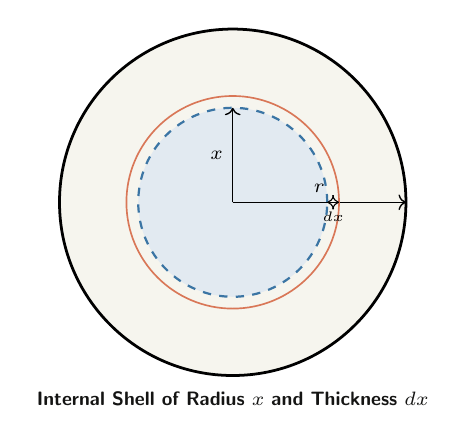
\begin{tikzpicture}[scale=1.0]
  \draw[line width=1.0pt, fill=AnthCardBG] (0,0) circle (2.2cm);
  \draw[line width=0.8pt, dashed, color=AnthBlue, fill=AnthBlue!15] (0,0) circle (1.2cm);
  \draw[line width=0.5pt, ->] (0,0) -- node[above, font=\scriptsize\sffamily]{$r$} (2.2,0);
  \draw[line width=0.5pt, ->] (0,0) -- node[left, font=\scriptsize\sffamily]{$x$} (0,1.2);
  \draw[line width=0.6pt, color=AnthOrange] (0,0) circle (1.35cm);
  \draw[line width=0.4pt, <->] (1.2,0) -- node[below, font=\tiny\sffamily]{$dx$} (1.35,0);
  \node[font=\scriptsize\sffamily\bfseries, color=AnthDark] at (0,-2.5) {Internal Shell of Radius $x$ and Thickness $dx$};
\end{tikzpicture}%
}
\end{center}
1. By Ampere's Circuital Law, the magnetic field intensity $H_x$ at an internal radius $x \le r$ enclosed by the path is:
\begin{equation}
  \oint H_x \cdot dl = I_x \implies H_x (2\pi x) = I \left( \frac{\pi x^2}{\pi r^2} \right) = I \left(\frac{x^2}{r^2}\right) \implies H_x = \frac{I x}{2\pi r^2} \quad [\text{A/m}]
\end{equation}
2. The magnetic flux density is $B_x = \mu_0 H_x = \frac{\mu_0 I x}{2\pi r^2}$ (assuming non-magnetic conductor $\mu_r = 1$, $\mu_0 = 4\pi \times 10^{-7}\,\text{H/m}$).\\
3. The differential flux per meter length in the tubular shell of thickness $dx$ is $d\Phi = B_x \cdot (1 \cdot dx) = \frac{\mu_0 I x}{2\pi r^2} dx$.\\
4. This flux links only the fraction of current inside radius $x$, i.e., $N_x = \frac{\pi x^2}{\pi r^2} = \frac{x^2}{r^2}$. The internal flux linkage is:
\begin{equation}
  \lambda_{\text{int}} = \int_{0}^{r} \left(\frac{x^2}{r^2}\right) d\Phi = \int_{0}^{r} \frac{\mu_0 I x^3}{2\pi r^4} dx = \frac{\mu_0 I}{2\pi r^4} \left[ \frac{x^4}{4} \right]_0^r = \frac{\mu_0 I}{8\pi} \quad [\text{Wb-t/m}]
\end{equation}
5. Hence, the internal inductance is constant and 	extbf{independent of conductor radius}:
\begin{equation}
  L_{\text{int}} = \frac{\lambda_{\text{int}}}{I} = \frac{\mu_0}{8\pi} = \frac{4\pi \times 10^{-7}}{8\pi} = \frac{1}{2} \times 10^{-7} \quad [\text{H/m}]
\end{equation}
\end{Deriv}

\begin{Deriv}[Derivation of External Flux Linkage ($\lambda_{\text{ext}}$)]
For the magnetic flux outside the conductor between the surface $r$ and an external distance $D$:
\begin{equation}
  H_x (2\pi x) = I \implies B_x = \frac{\mu_0 I}{2\pi x}
\end{equation}
Since all external flux links the entire current ($N=1$), the external flux linkage is:
\begin{equation}
  \lambda_{\text{ext}} = \int_{r}^{D} B_x dx = \int_{r}^{D} \frac{\mu_0 I}{2\pi x} dx = \frac{\mu_0 I}{2\pi} \ln\left(\frac{D}{r}\right) \quad [\text{Wb-t/m}]
\end{equation}
The external inductance is:
\begin{equation}
  L_{\text{ext}} = \frac{\mu_0}{2\pi} \ln\left(\frac{D}{r}\right) = 2 \times 10^{-7} \ln\left(\frac{D}{r}\right) \quad [\text{H/m}]
\end{equation}
\end{Deriv}

\concept{Total Inductance and the Fictitious Self-GMR Concept}
Combining the internal and external components:
\begin{equation}
  L_{\text{total}} = L_{\text{int}} + L_{\text{ext}} = 2 \times 10^{-7} \left[ \frac{1}{4} + \ln\left(\frac{D}{r}\right) \right] \quad [\text{H/m}]
\end{equation}
Using the mathematical identity $\frac{1}{4} = \ln(e^{1/4})$:
\begin{equation}
  L_{\text{total}} = 2 \times 10^{-7} \left[ \ln(e^{1/4}) + \ln\left(\frac{D}{r}\right) \right] = 2 \times 10^{-7} \ln\left(\frac{D}{r \cdot e^{-1/4}}\right)
\end{equation}
\begin{Def}[Self GMR ($r'$) of a Solid Conductor]
We define the 	extbf{effective fictitious radius} or 	extbf{Self Geometric Mean Radius (GMR / $D_s$)} as:
\begin{equation}
  r' = D_s = r \cdot e^{-1/4} = r \cdot e^{-0.25} \approx 0.7788 \cdot r
\end{equation}
By replacing the physical solid conductor of radius $r$ with an equivalent fictitious hollow, infinitely thin shell of radius $r'$, the internal inductance is seamlessly accounted for in the single logarithmic expression:
\begin{equation}
  L = 2 \times 10^{-7} \ln\left(\frac{D}{r'}\right) = 2 \times 10^{-7} \ln\left(\frac{D_m}{D_s}\right) \quad [\text{H/m}]
\end{equation}
\end{Def}

%% ─────────────────────────────────────────────────────────────────────────────
\subsection{Inductance of 3-Phase Single-Circuit Lines}

\begin{enumerate}
  \item \textbf{Symmetrical / Equilateral Spacing ($D_{12} = D_{23} = D_{31} = D$):}
    Due to symmetry, the flux linkages of all three phases are balanced:
    \begin{equation}
      L_{\text{phase}} = 2 \times 10^{-7} \ln\left(\frac{D}{r'}\right) \quad [\text{H/m/phase}]
    \end{equation}
  \item \textbf{Unsymmetrical Spacing with Transposition ($D_{12} \neq D_{23} \neq D_{31}$):}
    If conductors are not transposed, the three phases experience unequal induced voltages and unbalanced impedance drops. When the line is 	extbf{regularly transposed} (cyclically rotating conductor positions in 3 equal sections along the route), the average phase inductance is:
    \begin{equation}
      L_{\text{phase}} = 2 \times 10^{-7} \ln\left(\frac{D_{\text{eq}}}{r'}\right) = 2 \times 10^{-7} \ln\left(\frac{D_m}{D_s}\right) \quad [\text{H/m/phase}]
    \end{equation}
    where the equivalent mutual geometric mean distance is:
    \begin{equation}
      D_{\text{eq}} = D_m = \sqrt[3]{D_{12} \cdot D_{23} \cdot D_{31}}
    \end{equation}
\end{enumerate}

%% ─────────────────────────────────────────────────────────────────────────────
\clearpage
\subsection{Derivation of Inductance for Three-Phase Double-Circuit Lines}

\syllabusitem{Derivation of three phase double circuit line parameters (inductance and capacitance)}

A three-phase double-circuit line consists of two parallel circuits sharing the same transmission tower structure: Circuit 1 ($a, b, c$) and Circuit 2 ($a', b', c'$). To maintain balanced electrical characteristics and minimize total loop inductance, the conductors are transposed cyclically and arranged in an inverted hexagonal/vertical configuration.

\begin{center}
\resizebox{0.75\textwidth}{!}{%
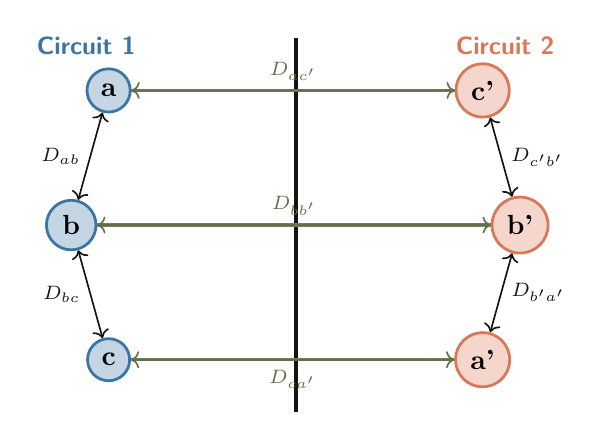
\begin{tikzpicture}[scale=0.95]
  %% Tower Cross-arm Representation
  \draw[line width=1.5pt, color=AnthDark] (0, 4.5) -- (0, -0.5);
  \draw[line width=1.2pt, color=AnthMidGray] (-2.5, 3.8) -- (2.5, 3.8);
  \draw[line width=1.2pt, color=AnthMidGray] (-3.0, 2.0) -- (3.0, 2.0);
  \draw[line width=1.2pt, color=AnthMidGray] (-2.5, 0.2) -- (2.5, 0.2);

  %% Conductors Circuit 1 (Left) & Circuit 2 (Right)
  \node[circle, draw=AnthBlue, fill=AnthBlue!30, line width=1.0pt, inner sep=3pt] (a) at (-2.5, 3.8) {\textbf{a}};
  \node[circle, draw=AnthBlue, fill=AnthBlue!30, line width=1.0pt, inner sep=3pt] (b) at (-3.0, 2.0) {\textbf{b}};
  \node[circle, draw=AnthBlue, fill=AnthBlue!30, line width=1.0pt, inner sep=3pt] (c) at (-2.5, 0.2) {\textbf{c}};

  \node[circle, draw=AnthOrange, fill=AnthOrange!30, line width=1.0pt, inner sep=3pt] (cp) at (2.5, 3.8) {\textbf{c'}};
  \node[circle, draw=AnthOrange, fill=AnthOrange!30, line width=1.0pt, inner sep=3pt] (bp) at (3.0, 2.0) {\textbf{b'}};
  \node[circle, draw=AnthOrange, fill=AnthOrange!30, line width=1.0pt, inner sep=3pt] (ap) at (2.5, 0.2) {\textbf{a'}};

  %% Dimension Labels
  \draw[<->, line width=0.6pt, color=AnthGreen] (a) -- node[above, font=\scriptsize\sffamily]{$D_{a c'}$} (cp);
  \draw[<->, line width=0.6pt, color=AnthGreen] (b) -- node[above, font=\scriptsize\sffamily]{$D_{b b'}$} (bp);
  \draw[<->, line width=0.6pt, color=AnthGreen] (c) -- node[below, font=\scriptsize\sffamily]{$D_{c a'}$} (ap);

  \draw[<->, line width=0.6pt, color=AnthDark] (a) -- node[left, font=\scriptsize\sffamily]{$D_{ab}$} (b);
  \draw[<->, line width=0.6pt, color=AnthDark] (b) -- node[left, font=\scriptsize\sffamily]{$D_{bc}$} (c);
  \draw[<->, line width=0.6pt, color=AnthDark] (cp) -- node[right, font=\scriptsize\sffamily]{$D_{c'b'}$} (bp);
  \draw[<->, line width=0.6pt, color=AnthDark] (bp) -- node[right, font=\scriptsize\sffamily]{$D_{b'a'}$} (ap);

  \node[font=\small\sffamily\bfseries, color=AnthBlue] at (-2.8, 4.4) {Circuit 1};
  \node[font=\small\sffamily\bfseries, color=AnthOrange] at (2.8, 4.4) {Circuit 2};
\end{tikzpicture}%
}
\end{center}

\begin{Deriv}[Complete Step-by-Step Derivation of Inductance for 3-$\Phi$ Double Circuit]
Let each conductor have physical radius $r$, fictitious self-radius $r' = 0.7788r$, and let the line carry balanced 3-phase currents:
\begin{equation}
  I_a + I_b + I_c = 0
\end{equation}
Because the two circuits operate in parallel, the current divides equally between paired conductors:
$I_a = I_{a'} = \frac{I_A}{2}$, $I_b = I_{b'} = \frac{I_B}{2}$, $I_c = I_{c'} = \frac{I_C}{2}$.

\concept{Step 1: Evaluation of Self GMD ($D_s$ / GMR of each phase)}
For Phase A, which consists of parallel conductors $a$ and $a'$:
\begin{equation}
  D_{sa} = \sqrt[4]{D_{aa} \cdot D_{aa'} \cdot D_{a'a} \cdot D_{a'a'}} = \sqrt[4]{r' \cdot D_{aa'} \cdot D_{a'a} \cdot r'} = \sqrt{r' \cdot D_{aa'}}
\end{equation}
Similarly, for Phase B (conductors $b, b'$) and Phase C (conductors $c, c'$):
\begin{align}
  D_{sb} &= \sqrt{r' \cdot D_{bb'}} \\
  D_{sc} &= \sqrt{r' \cdot D_{cc'}}
\end{align}
The equivalent composite 	extbf{Self GMD ($D_s$)} of the transposed three-phase system is the geometric mean:
\begin{equation}
  D_s = \sqrt[3]{D_{sa} \cdot D_{sb} \cdot D_{sc}} = \sqrt[3]{\sqrt{r' D_{aa'}} \cdot \sqrt{r' D_{bb'}} \cdot \sqrt{r' D_{cc'}}}
\end{equation}

\concept{Step 2: Evaluation of Mutual GMD ($D_m$ between phase pairs)}
The mutual distance between Phase A ($a, a'$) and Phase B ($b, b'$) is the geometric mean of all 4 mutual distances:
\begin{equation}
  D_{ab} = \sqrt[4]{D_{ab} \cdot D_{ab'} \cdot D_{a'b} \cdot D_{a'b'}}
\end{equation}
Similarly, between Phase B and Phase C, and between Phase C and Phase A:
\begin{align}
  D_{bc} &= \sqrt[4]{D_{bc} \cdot D_{bc'} \cdot D_{b'c} \cdot D_{b'c'}} \\
  D_{ca} &= \sqrt[4]{D_{ca} \cdot D_{ca'} \cdot D_{c'a} \cdot D_{c'a'}}
\end{align}
The equivalent composite 	extbf{Mutual GMD ($D_m$)} of the transposed three-phase system is:
\begin{equation}
  D_m = \sqrt[3]{D_{ab} \cdot D_{bc} \cdot D_{ca}}
\end{equation}

\concept{Step 3: Final Phase Inductance Formula}
Applying the GMD-GMR method, the total inductance per phase per unit length is:
\begin{equation}
  L_{\text{phase}} = 2 \times 10^{-7} \ln\left( \frac{D_m}{D_s} \right) \quad [\text{H/m/phase}]
\end{equation}
Or equivalently in millihenries per kilometer:
\begin{equation}
  L_{\text{phase}} = 0.2 \ln\left( \frac{D_m}{D_s} \right) \quad [\text{mH/km/phase}]
\end{equation}
\end{Deriv}

\begin{Tip}[Why Inverted Phase Configuration ($a-b-c$ vs $c'-b'-a'$) is Preferred]
Notice in the tower schematic that Circuit 1 has vertical arrangement $a-b-c$ while Circuit 2 is inverted to $c'-b'-a'$. This maximizes the diagonal separation between identical phases ($D_{aa'}, D_{cc'}$), which \textbf{maximizes the composite Self GMR ($D_s$)} and minimizes the mutual coupling, thereby reducing the total series inductive reactance by \textbf{10--20\%} compared to non-inverted layouts.
\end{Tip}

%% ─────────────────────────────────────────────────────────────────────────────
\subsection{Line Capacitance Fundamentals}

\concept{Electric Field and Potential Difference}
By Gauss's Law, a long cylindrical conductor of radius $r$ carrying a uniform surface charge $q\,\text{C/m}$ creates a radial electric field in surrounding dielectric medium of permittivity $\epsilon = \epsilon_0 \epsilon_r$ ($\epsilon_0 \approx 8.854 \times 10^{-12}\,\text{F/m}$):
\begin{equation}
  E_x = \frac{q}{2\pi \epsilon x} \quad [\text{V/m}]
\end{equation}
The electric potential difference between radius $r$ and an external point at distance $D$ is:
\begin{equation}
  V = \int_{r}^{D} E_x dx = \int_{r}^{D} \frac{q}{2\pi \epsilon x} dx = \frac{q}{2\pi \epsilon} \ln\left(\frac{D}{r}\right) \quad [\text{Volts}]
\end{equation}

\concept{Capacitance of a Single-Phase 2-Wire Line}
For two parallel conductors separated by center-to-center distance $D$ carrying charges $+q$ and $-q$:
\begin{equation}
  V_{ab} = \frac{q}{\pi \epsilon_0} \ln\left(\frac{D}{r}\right) \implies C_{ab} = \frac{q}{V_{ab}} = \frac{\pi \epsilon_0}{\ln(D/r)} \quad [\text{F/m}]
\end{equation}
The line-to-neutral (or line-to-ground) capacitance is double the line-to-line value:
\begin{equation}
  C_n = 2 C_{ab} = \frac{2\pi \epsilon_0}{\ln(D/r)} \quad [\text{F/m}]
\end{equation}

\begin{Warn}[Critical Distinction: Radius in Inductance vs. Capacitance]
In inductance calculations, the magnetic flux penetrating the conductor interior requires using the fictitious radius $r' = 0.7788r$. In capacitance calculations, electrostatic charge resides 	extbf{strictly on the outer physical conductor surface} ($E=0$ inside conductor), so 	extbf{always use the actual physical radius $r$} (do NOT apply the $0.7788$ factor!).
\end{Warn}

%% ─────────────────────────────────────────────────────────────────────────────
\clearpage
\subsection{Derivation of Capacitance for Three-Phase Double-Circuit Lines}

\begin{Deriv}[Complete Step-by-Step Derivation of Capacitance for 3-$\Phi$ Double Circuit]
Consider a transposed 3-phase double-circuit line carrying charges $q_a, q_b, q_c$ per phase such that:
\begin{equation}
  q_a + q_b + q_c = 0
\end{equation}
The charge on each phase divides equally between the two parallel conductors:
$q_a = q_{a'} = \frac{q_A}{2}$, $q_b = q_{b'} = \frac{q_B}{2}$, $q_c = q_{c'} = \frac{q_C}{2}$.

\concept{Step 1: Evaluation of Capacitive Self GMR ($D_{sc}$)}
For Phase A, using the actual conductor radius $r$:
\begin{equation}
  D_{sca} = \sqrt{r \cdot D_{aa'}}
\end{equation}
Similarly for Phases B and C:
\begin{align}
  D_{scb} &= \sqrt{r \cdot D_{bb'}} \\
  D_{scc} &= \sqrt{r \cdot D_{cc'}}
\end{align}
The equivalent composite 	extbf{Capacitive Self GMD ($D_{sc}$)} of the transposed system is:
\begin{equation}
  D_{sc} = \sqrt[3]{D_{sca} \cdot D_{scb} \cdot D_{scc}} = \sqrt[3]{\sqrt{r D_{aa'}} \cdot \sqrt{r D_{bb'}} \cdot \sqrt{r D_{cc'}}}
\end{equation}

\concept{Step 2: Evaluation of Mutual GMD ($D_m$)}
The mutual geometric mean distance $D_m$ is identical to that used in inductance calculations:
\begin{equation}
  D_{ab} = \sqrt[4]{D_{ab} D_{ab'} D_{a'b} D_{a'b'}}, \quad D_{bc} = \sqrt[4]{D_{bc} D_{bc'} D_{b'c} D_{b'c'}}, \quad D_{ca} = \sqrt[4]{D_{ca} D_{ca'} D_{c'a} D_{c'a'}}
\end{equation}
\begin{equation}
  D_m = \sqrt[3]{D_{ab} \cdot D_{bc} \cdot D_{ca}}
\end{equation}

\concept{Step 3: Final Line-to-Neutral Capacitance Formula}
The line-to-neutral capacitance per unit length of the transposed double-circuit line is:
\begin{equation}
  C_n = \frac{2\pi \epsilon_0}{\ln\left( \frac{D_m}{D_{sc}} \right)} \quad [\text{F/m/phase}]
\end{equation}
Or equivalently in microfarads per kilometer:
\begin{equation}
  C_n = \frac{0.0242}{\log_{10}\left( \frac{D_m}{D_{sc}} \right)} \quad [\mu\text{F/km/phase}]
\end{equation}
\end{Deriv}

\concept{Effect of Earth on Transmission Line Capacitance (Method of Images)}
The earth surface acts as a conducting equipotential plane ($V=0$). By Kelvin's 	extbf{Method of Images}, the boundary condition at the earth plane is satisfied by replacing the earth with a fictitious image conductor at depth $h$ carrying charge $-q$.

\begin{center}
\resizebox{0.55\textwidth}{!}{%
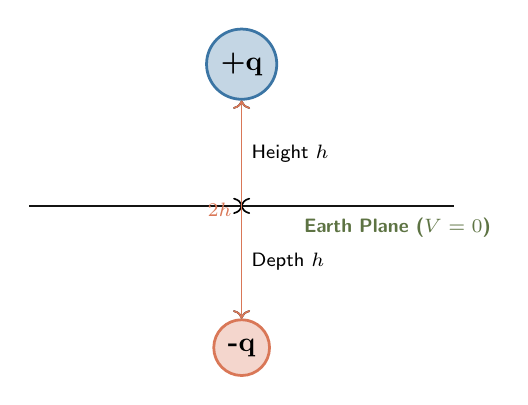
\begin{tikzpicture}[scale=0.9]
  \draw[line width=1.0pt, color=AnthDark] (-3,0) -- (3,0);
  \node[font=\scriptsize\sffamily\bfseries, color=AnthGreen] at (2.2, -0.3) {Earth Plane ($V=0$)};
  
  \node[circle, draw=AnthBlue, fill=AnthBlue!30, line width=1.0pt, inner sep=3pt] (cond) at (0, 2.0) {\textbf{+q}};
  \node[circle, draw=AnthOrange, fill=AnthOrange!30, line width=1.0pt, inner sep=3pt] (img) at (0, -2.0) {\textbf{-q}};
  
  \draw[<->, line width=0.6pt, dashed] (cond) -- node[right, font=\scriptsize\sffamily]{Height $h$} (0,0);
  \draw[<->, line width=0.6pt, dashed] (img) -- node[right, font=\scriptsize\sffamily]{Depth $h$} (0,0);
  \draw[<->, line width=0.6pt, color=AnthOrange] (cond) -- node[left, font=\scriptsize\sffamily]{$2h$} (img);
\end{tikzpicture}%
}
\end{center}

Including the image charges modifies the capacitance formula to:
\begin{equation}
  C_n = \frac{2\pi \epsilon_0}{\ln\left(\frac{D}{r}\right) - \ln\left(\sqrt{1 + \left(\frac{D}{2h}\right)^2}\right)} \quad [\text{F/m}]
\end{equation}
Because the denominator is slightly decreased, the presence of the earth 	extbf{increases the line-to-neutral capacitance} (typically by $1-5\%$), though for typical high-voltage lines with large clearance ($h \gg D$), this effect is small.

%% ─────────────────────────────────────────────────────────────────────────────
\clearpage
\section{Transmission Line Modelling and Two-Port ABCD Parameters}
%% ─────────────────────────────────────────────────────────────────────────────

\syllabusitem{Transmission line modelling - classifications (concept only) – transmission line as two port network – derivation and calculation of ABCD parameters (derivation and numerical problems)}

\subsection{Classification of Transmission Lines}

Transmission lines are classified into three distinct categories based on their physical length $l$ and operating voltage $V$:

\begin{center}
\small
\begin{tabularx}{\textwidth}{L{2.5cm} C{2.2cm} C{2.2cm} L{3.5cm} X}
  \rowcolor{AnthDark}
  \color{white}\textbf{Classification} & \color{white}\textbf{Length ($l$)} & \color{white}\textbf{Voltage ($V$)} & \color{white}\textbf{Capacitance Treatment} & \color{white}\textbf{Mathematical Model} \\
  \rowcolor{AnthCardBG} \textbf{Short Line} & $< 80\,\text{km}$ & $< 20\,\text{kV}$ & Neglected entirely & Simple lumped series $R-L$ impedance \\
  \textbf{Medium Line} & $80 - 250\,\text{km}$ & $20 - 100\,\text{kV}$ & Lumped at discrete nodes & Nominal-T or Nominal-$\pi$ networks \\
  \rowcolor{AnthCardBG} \textbf{Long Line} & $> 250\,\text{km}$ & $> 100\,\text{kV}$ & Uniformly distributed & Rigorous distributed hyperbolic equations \\
\end{tabularx}
\end{center}

%% ─────────────────────────────────────────────────────────────────────────────
\subsection{The Transmission Line as a Two-Port Network}

A transmission line is a linear, passive, and bilateral electrical network with two input terminals (Sending End, subscript $s$) and two output terminals (Receiving End, subscript $r$).

\begin{center}
\resizebox{0.75\textwidth}{!}{%
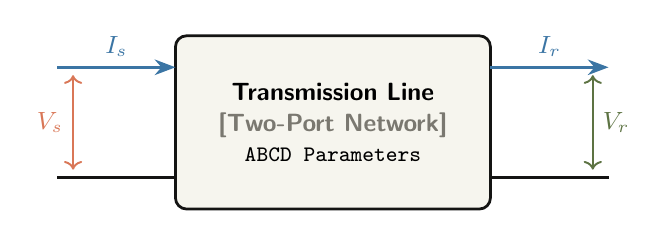
\begin{tikzpicture}[
  block/.style={rectangle, draw=AnthDark, fill=AnthCardBG, rounded corners=4pt, line width=1.0pt, minimum width=4.0cm, minimum height=2.2cm, align=center, font=\small\sffamily\bfseries},
  arrow/.style={-{Stealth[scale=1.0]}, line width=1.0pt, color=AnthBlue}
]
  \node[block] (box) {Transmission Line\\ \small\sffamily\color{AnthMidGray}[Two-Port Network]\\ \footnotesize\ttfamily ABCD Parameters};
  
  %% Sending End
  \draw[arrow] (-3.5, 0.7) -- node[above, font=\small\sffamily]{$I_s$} (-2.0, 0.7);
  \draw[line width=1.0pt, color=AnthDark] (-3.5, -0.7) -- (-2.0, -0.7);
  \draw[<->, line width=0.7pt, color=AnthOrange] (-3.3, 0.6) -- node[left, font=\small\sffamily]{$V_s$} (-3.3, -0.6);

  %% Receiving End
  \draw[arrow] (2.0, 0.7) -- node[above, font=\small\sffamily]{$I_r$} (3.5, 0.7);
  \draw[line width=1.0pt, color=AnthDark] (2.0, -0.7) -- (3.5, -0.7);
  \draw[<->, line width=0.7pt, color=AnthGreen] (3.3, 0.6) -- node[right, font=\small\sffamily]{$V_r$} (3.3, -0.6);
\end{tikzpicture}%
}
\end{center}

\concept{The Governing Matrix Equations}
\begin{equation}
  \begin{bmatrix} V_s \\ I_s \end{bmatrix} = \begin{bmatrix} A & B \\ C & D \end{bmatrix} \begin{bmatrix} V_r \\ I_r \end{bmatrix}
\end{equation}
\begin{align}
  V_s &= A V_r + B I_r \\
  I_s &= C V_r + D I_r
\end{align}

\concept{Physical Definitions \& Dimensions of ABCD Parameters}
\begin{enumerate}
  \item $A = \left.\frac{V_s}{V_r}\right|_{I_r=0}$: 	extbf{Open-circuit reverse voltage ratio} (Dimensionless).
  \item $B = \left.\frac{V_s}{I_r}\right|_{V_r=0}$: 	extbf{Short-circuit transfer impedance} (Units: Ohms, $\Omega$).
  \item $C = \left.\frac{I_s}{V_r}\right|_{I_r=0}$: 	extbf{Open-circuit transfer admittance} (Units: Siemens or $\mho$).
  \item $D = \left.\frac{I_s}{I_r}\right|_{V_r=0}$: 	extbf{Short-circuit reverse current ratio} (Dimensionless).
\end{enumerate}

\begin{Note}[Fundamental Network Conditions]
\begin{itemize}
  \item \textbf{Condition for Symmetry:} A transmission line looks identical viewed from either terminal pair:
    \begin{equation}
      A = D
    \end{equation}
  \item \textbf{Condition for Reciprocity:} For any linear, bilateral, passive network:
    \begin{equation}
      A D - B C = 1
    \end{equation}
\end{itemize}
\end{Note}

%% ─────────────────────────────────────────────────────────────────────────────
\subsection{Derivation of ABCD Parameters for Line Models}

Let total series line impedance be $Z = R + j X_L = R + j\omega L$, and total line shunt admittance be $Y = G + j B_C = j\omega C$ (neglecting conductance $G=0$).

\begin{Deriv}[1. Short Transmission Line Model ($< 80\,\text{km}$)]
In short lines, shunt capacitance is negligible ($Y = 0$).
\begin{center}
\resizebox{0.55\textwidth}{!}{%
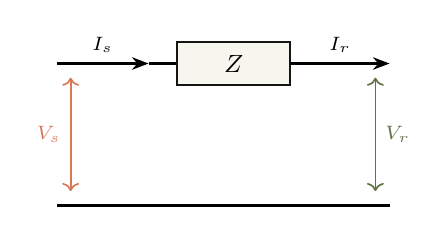
\begin{tikzpicture}[scale=0.9]
  \draw[line width=1.0pt, -{Stealth[scale=0.8]}] (-2.5, 1.0) -- node[above, font=\scriptsize\sffamily]{$I_s$} (-1.2, 1.0);
  \draw[line width=1.0pt] (-1.2, 1.0) -- (-0.8, 1.0);
  \draw[draw=AnthDark, fill=AnthCardBG, line width=0.8pt] (-0.8, 0.7) rectangle (0.8, 1.3) node[midway, font=\small\sffamily\bfseries]{$Z$};
  \draw[line width=1.0pt, -{Stealth[scale=0.8]}] (0.8, 1.0) -- node[above, font=\scriptsize\sffamily]{$I_r$} (2.2, 1.0);
  \draw[line width=1.0pt] (-2.5, -1.0) -- (2.2, -1.0);
  \draw[<->, line width=0.6pt, color=AnthOrange] (-2.3, 0.8) -- node[left, font=\scriptsize\sffamily]{$V_s$} (-2.3, -0.8);
  \draw[<->, line width=0.6pt, color=AnthGreen] (2.0, 0.8) -- node[right, font=\scriptsize\sffamily]{$V_r$} (2.0, -0.8);
\end{tikzpicture}%
}
\end{center}
Applying KVL and KCL:
\begin{align}
  V_s &= V_r + I_r Z = (1) V_r + (Z) I_r \\
  I_s &= I_r = (0) V_r + (1) I_r
\end{align}
Comparing with standard ABCD equations:
\begin{equation}
  A = 1, \quad B = Z, \quad C = 0, \quad D = 1
\end{equation}
\emph{Verification:} $AD - BC = (1)(1) - (Z)(0) = 1$ \quad \checkmark
\end{Deriv}

\begin{Deriv}[2. Medium Line: Nominal-T Method ($80 - 250\,\text{km}$)]
In the Nominal-T network, total series impedance is split equally into two halves ($Z/2$), and the entire shunt admittance $Y$ is lumped at the center node.
\begin{center}
\resizebox{0.75\textwidth}{!}{%
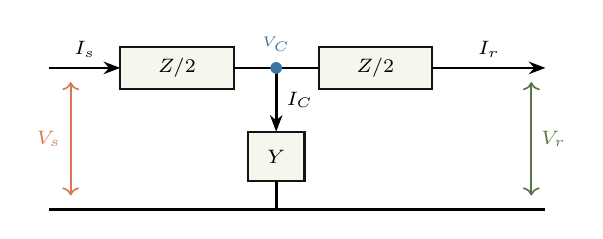
\begin{tikzpicture}[scale=0.9]
  \draw[line width=1.0pt, -{Stealth[scale=0.8]}] (-3.8, 1.0) -- node[above, font=\scriptsize\sffamily]{$I_s$} (-2.8, 1.0);
  \draw[draw=AnthDark, fill=AnthCardBG, line width=0.8pt] (-2.8, 0.7) rectangle (-1.2, 1.3) node[midway, font=\scriptsize\sffamily\bfseries]{$Z/2$};
  \draw[line width=1.0pt] (-1.2, 1.0) -- (0, 1.0);
  \draw[draw=AnthDark, fill=AnthCardBG, line width=0.8pt] (0, 0.7) rectangle (1.6, 1.3) node[midway, font=\scriptsize\sffamily\bfseries]{$Z/2$};
  \draw[line width=1.0pt, -{Stealth[scale=0.8]}] (1.6, 1.0) -- node[above, font=\scriptsize\sffamily]{$I_r$} (3.2, 1.0);

  %% Shunt Branch
  \draw[line width=1.0pt, -{Stealth[scale=0.8]}] (-0.6, 1.0) -- node[right, font=\scriptsize\sffamily]{$I_C$} (-0.6, 0.1);
  \draw[draw=AnthDark, fill=AnthCardBG, line width=0.8pt] (-1.0, -0.6) rectangle (-0.2, 0.1) node[midway, font=\scriptsize\sffamily\bfseries]{$Y$};
  \draw[line width=1.0pt] (-0.6, -0.6) -- (-0.6, -1.0);

  \draw[line width=1.0pt] (-3.8, -1.0) -- (3.2, -1.0);
  \draw[<->, line width=0.6pt, color=AnthOrange] (-3.5, 0.8) -- node[left, font=\scriptsize\sffamily]{$V_s$} (-3.5, -0.8);
  \draw[<->, line width=0.6pt, color=AnthGreen] (3.0, 0.8) -- node[right, font=\scriptsize\sffamily]{$V_r$} (3.0, -0.8);
  \node[circle, fill=AnthBlue, inner sep=1.5pt] at (-0.6, 1.0) {};
  \node[above, font=\tiny\sffamily, color=AnthBlue] at (-0.6, 1.1) {$V_C$};
\end{tikzpicture}%
}
\end{center}
1. Voltage at central junction: $V_C = V_r + I_r \left(\frac{Z}{2}\right)$.\\
2. Current through central shunt capacitor: $I_C = Y V_C = Y \left[ V_r + I_r \left(\frac{Z}{2}\right) \right] = Y V_r + \frac{YZ}{2} I_r$.\\
3. Sending-end current:
\begin{equation}
  I_s = I_r + I_C = Y V_r + \left(1 + \frac{YZ}{2}\right) I_r \implies C = Y, \quad D = 1 + \frac{YZ}{2}
\end{equation}
4. Sending-end voltage:
\begin{align}
  V_s &= V_C + I_s \left(\frac{Z}{2}\right) = \left[ V_r + I_r \left(\frac{Z}{2}\right) \right] + \left[ Y V_r + \left(1 + \frac{YZ}{2}\right) I_r \right] \frac{Z}{2} \nonumber\\
      &= \left(1 + \frac{YZ}{2}\right) V_r + Z \left(1 + \frac{YZ}{4}\right) I_r \implies A = 1 + \frac{YZ}{2}, \quad B = Z \left(1 + \frac{YZ}{4}\right)
\end{align}
\emph{Verification:} $AD - BC = \left(1 + \frac{YZ}{2}\right)^2 - Z\left(1 + \frac{YZ}{4}\right)Y = 1 + YZ + \frac{Y^2 Z^2}{4} - YZ - \frac{Y^2 Z^2}{4} = 1$ \quad \checkmark
\end{Deriv}

\begin{Deriv}[3. Medium Line: Nominal-$\pi$ Method ($80 - 250\,\text{km}$)]
In the Nominal-$\pi$ network, series impedance $Z$ is concentrated in the middle branch, and shunt admittance is split equally into two halves ($Y/2$) at sending and receiving terminals.
\begin{center}
\resizebox{0.75\textwidth}{!}{%
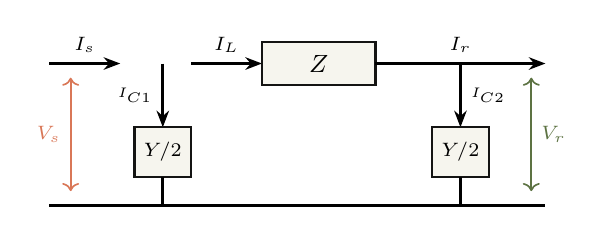
\begin{tikzpicture}[scale=0.9]
  \draw[line width=1.0pt, -{Stealth[scale=0.8]}] (-3.8, 1.0) -- node[above, font=\scriptsize\sffamily]{$I_s$} (-2.8, 1.0);
  \draw[line width=1.0pt, -{Stealth[scale=0.8]}] (-1.8, 1.0) -- node[above, font=\scriptsize\sffamily]{$I_L$} (-0.8, 1.0);
  \draw[draw=AnthDark, fill=AnthCardBG, line width=0.8pt] (-0.8, 0.7) rectangle (0.8, 1.3) node[midway, font=\small\sffamily\bfseries]{$Z$};
  \draw[line width=1.0pt, -{Stealth[scale=0.8]}] (0.8, 1.0) -- node[above, font=\scriptsize\sffamily]{$I_r$} (3.2, 1.0);

  %% Shunt 1 (Sending)
  \draw[line width=1.0pt, -{Stealth[scale=0.8]}] (-2.2, 1.0) -- node[left, font=\tiny\sffamily]{$I_{C1}$} (-2.2, 0.1);
  \draw[draw=AnthDark, fill=AnthCardBG, line width=0.8pt] (-2.6, -0.6) rectangle (-1.8, 0.1) node[midway, font=\scriptsize\sffamily\bfseries]{$Y/2$};
  \draw[line width=1.0pt] (-2.2, -0.6) -- (-2.2, -1.0);

  %% Shunt 2 (Receiving)
  \draw[line width=1.0pt, -{Stealth[scale=0.8]}] (2.0, 1.0) -- node[right, font=\tiny\sffamily]{$I_{C2}$} (2.0, 0.1);
  \draw[draw=AnthDark, fill=AnthCardBG, line width=0.8pt] (1.6, -0.6) rectangle (2.4, 0.1) node[midway, font=\scriptsize\sffamily\bfseries]{$Y/2$};
  \draw[line width=1.0pt] (2.0, -0.6) -- (2.0, -1.0);

  \draw[line width=1.0pt] (-3.8, -1.0) -- (3.2, -1.0);
  \draw[<->, line width=0.6pt, color=AnthOrange] (-3.5, 0.8) -- node[left, font=\scriptsize\sffamily]{$V_s$} (-3.5, -0.8);
  \draw[<->, line width=0.6pt, color=AnthGreen] (3.0, 0.8) -- node[right, font=\scriptsize\sffamily]{$V_r$} (3.0, -0.8);
\end{tikzpicture}%
}
\end{center}
1. Current in receiving shunt branch: $I_{C2} = \left(\frac{Y}{2}\right) V_r$.\\
2. Current through series impedance $Z$: $I_L = I_r + I_{C2} = I_r + \left(\frac{Y}{2}\right) V_r$.\\
3. Sending-end voltage:
\begin{equation}
  V_s = V_r + I_L Z = V_r + \left(I_r + \frac{Y}{2} V_r\right) Z = \left(1 + \frac{YZ}{2}\right) V_r + Z I_r \implies A = 1 + \frac{YZ}{2}, \quad B = Z
\end{equation}
4. Current in sending shunt branch: $I_{C1} = \left(\frac{Y}{2}\right) V_s = \frac{Y}{2} \left[ \left(1 + \frac{YZ}{2}\right) V_r + Z I_r \right]$.\\
5. Sending-end current:
\begin{align}
  I_s &= I_L + I_{C1} = \left( I_r + \frac{Y}{2} V_r \right) + \frac{Y}{2} \left(1 + \frac{YZ}{2}\right) V_r + \frac{YZ}{2} I_r \nonumber\\
      &= Y \left(1 + \frac{YZ}{4}\right) V_r + \left(1 + \frac{YZ}{2}\right) I_r \implies C = Y \left(1 + \frac{YZ}{4}\right), \quad D = 1 + \frac{YZ}{2}
\end{align}
\emph{Verification:} $AD - BC = \left(1 + \frac{YZ}{2}\right)^2 - Z \cdot Y\left(1 + \frac{YZ}{4}\right) = 1$ \quad \checkmark
\end{Deriv}

\begin{Tip}[Master Comparison of ABCD Parameters]
\begin{center}
\small
\begin{tabularx}{\textwidth}{L{2.5cm} C{2.2cm} C{2.5cm} C{2.8cm} C{2.2cm}}
  \rowcolor{AnthDark}
  \color{white}\textbf{Model} & \color{white}\textbf{A} & \color{white}\textbf{B} & \color{white}\textbf{C} & \color{white}\textbf{D} \\
  \rowcolor{AnthCardBG} \textbf{Short Line} & $1$ & $Z$ & $0$ & $1$ \\
  \textbf{Nominal-T} & $1 + \frac{YZ}{2}$ & $Z\left(1 + \frac{YZ}{4}\right)$ & $Y$ & $1 + \frac{YZ}{2}$ \\
  \rowcolor{AnthCardBG} \textbf{Nominal-$\pi$} & $1 + \frac{YZ}{2}$ & $Z$ & $Y\left(1 + \frac{YZ}{4}\right)$ & $1 + \frac{YZ}{2}$ \\
  \textbf{Long Line} & $\cosh(\gamma l)$ & $Z_c \sinh(\gamma l)$ & $\frac{1}{Z_c}\sinh(\gamma l)$ & $\cosh(\gamma l)$ \\
\end{tabularx}
\end{center}
\end{Tip}

%% ─────────────────────────────────────────────────────────────────────────────
\subsection{Voltage Regulation and Transmission Efficiency}

\concept{1. Percentage Voltage Regulation ($VR\%$)}
Voltage regulation is the percentage change in receiving-end voltage when full rated load at a specified power factor is dropped to zero, keeping sending-end voltage constant.
\begin{equation}
  \text{At No Load } (I_r = 0): \quad V_s = A V_{r0} \implies V_{r0} = \frac{V_s}{A}
\end{equation}
\begin{equation}
  \% VR = \frac{|V_{r0}| - |V_r|}{|V_r|} \times 100\% = \frac{\left|\frac{V_s}{A}\right| - |V_r|}{|V_r|} \times 100\%
\end{equation}
For short lines where $A=1$, $\% VR = \frac{|V_s| - |V_r|}{|V_r|} \times 100\% \approx \frac{I_r (R \cos\phi_r \pm X \sin\phi_r)}{|V_r|} \times 100\%$ ($+$ for lagging, $-$ for leading).

\concept{2. Transmission Efficiency ($\eta\%$)}
\begin{equation}
  \eta = \frac{\text{Total 3-Phase Active Power Received ($P_r$)}}{\text{Total 3-Phase Active Power Supplied ($P_s$)}} \times 100\%
\end{equation}
\begin{equation}
  P_r = \sqrt{3} |V_{r,\text{line}}| |I_r| \cos\phi_r = 3 |V_{r,\text{ph}}| |I_r| \cos\phi_r
\end{equation}
\begin{equation}
  P_s = 3 \operatorname{Re}\left( V_{s,\text{ph}} \cdot I_s^* \right) = P_r + 3 |I_{\text{line}}|^2 R
\end{equation}

%% ─────────────────────────────────────────────────────────────────────────────
\clearpage
\section{Operational Phenomena in Transmission Lines}
%% ─────────────────────────────────────────────────────────────────────────────

\syllabusitem{Skin Effect \& Ferranti Effect – Corona (qualitative study only) – Surge Impedance Loading}

\subsection{The Skin Effect}

\concept{Physical Mechanism \& Skin Depth}
Under direct current (DC), current density $J$ is uniformly distributed over the entire cross-section of a conductor. Under alternating current (AC), the alternating magnetic flux induces concentric eddy currents that oppose current flow at the center and reinforce it at the surface. Consequently, current concentrates in a thin outer layer or 	extbf{skin}.

\begin{center}
\resizebox{0.7\textwidth}{!}{%
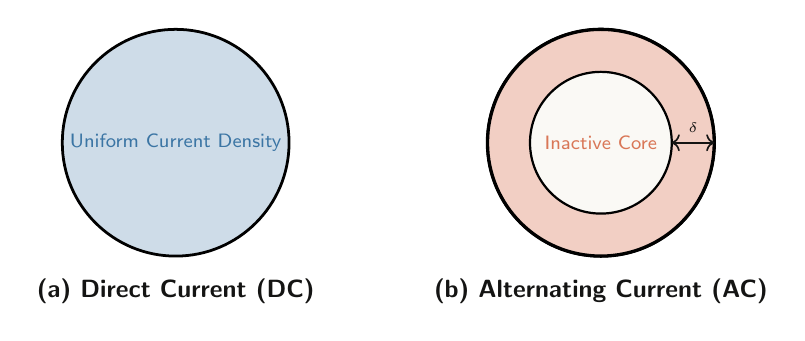
\begin{tikzpicture}[scale=0.9]
  %% DC Conductor
  \draw[line width=1.0pt, fill=AnthBlue!25] (-3,0) circle (1.6cm);
  \node[font=\small\sffamily\bfseries, color=AnthDark] at (-3, -2.1) {(a) Direct Current (DC)};
  \node[font=\scriptsize\sffamily, color=AnthBlue] at (-3, 0) {Uniform Current Density};

  %% AC Conductor
  \draw[line width=1.0pt, fill=AnthCardBG] (3,0) circle (1.6cm);
  \draw[line width=1.2pt, fill=AnthOrange!35] (3,0) circle (1.6cm);
  \draw[line width=0.8pt, fill=AnthLight] (3,0) circle (1.0cm);
  \draw[<->, line width=0.6pt, color=AnthDark] (4.0, 0) -- node[above, font=\tiny\sffamily]{$\delta$} (4.6, 0);
  \node[font=\small\sffamily\bfseries, color=AnthDark] at (3, -2.1) {(b) Alternating Current (AC)};
  \node[font=\scriptsize\sffamily, color=AnthOrange] at (3, 0) {Inactive Core};
\end{tikzpicture}%
}
\end{center}

The effective depth to which AC current penetrates before decaying to $1/e$ ($\approx 36.8\%$) of its surface value is the 	extbf{skin depth ($\delta$)}:
\begin{equation}
  \delta = \sqrt{\frac{\rho}{\pi f \mu}} = \sqrt{\frac{1}{\pi f \mu \sigma}} \quad [\text{meters}]
\end{equation}

\concept{Factors Influencing Skin Effect}
\begin{enumerate}
  \item \textbf{Supply Frequency ($f$):} Skin effect increases with higher frequency ($\propto \sqrt{f}$).
  \item \textbf{Conductor Diameter ($d$):} Increases rapidly with conductor cross-sectional area ($\propto d^2$). Negligible for wire diameters $<1\,\text{cm}$ at 50 Hz.
  \item \textbf{Permeability ($\mu$):} Higher magnetic permeability increases internal flux linkages.
  \item \textbf{Mitigation:} Using stranded ACSR conductors where the non-conducting steel core occupies the inactive central region, while high-conductivity aluminum occupies the outer perimeter.
\end{enumerate}

%% ─────────────────────────────────────────────────────────────────────────────
\subsection{The Ferranti Effect}

\concept{The Paradox of No-Load Voltage Rise}
In 1890, British engineer Sebastian Ziani de Ferranti observed that on medium and long unloaded high-voltage transmission lines, the 	extbf{receiving-end voltage exceeds the sending-end voltage ($V_r > V_s$)}.

\concept{Mathematical Derivation of Ferranti Rise}
Under no-load or light-load conditions, receiving-end load current $I_r \approx 0$. The line draws a pure leading capacitive charging current:
\begin{equation}
  I_c = j \omega C V_r
\end{equation}
This charging current flows through distributed series inductance $L$. Neglecting line resistance ($R \approx 0$):
\begin{equation}
  V_s = V_r + I_c (j X_L) = V_r + (j \omega C V_r)(j \omega L) = V_r - \omega^2 L C V_r = V_r \left( 1 - \omega^2 L C \right)
\end{equation}
Because $\omega^2 L C > 0$, it directly follows that $V_s < V_r$, or:
\begin{equation}
  \Delta V = V_r - V_s = V_r \cdot \omega^2 L C \approx \frac{V_r \cdot \omega^2 l^2 L_0 C_0}{2} > 0
\end{equation}

\begin{center}
\resizebox{0.55\textwidth}{!}{%
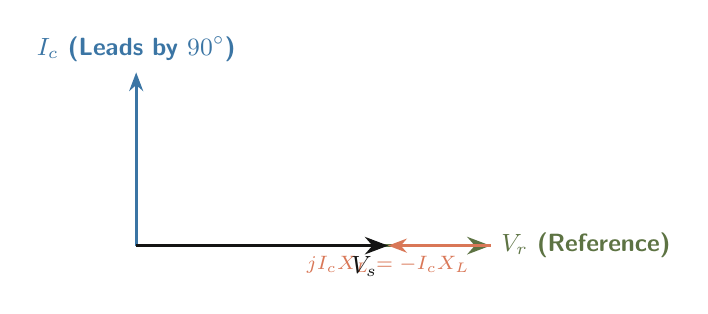
\begin{tikzpicture}[scale=1.0]
  \draw[line width=1.2pt, -{Stealth[scale=1.0]}, color=AnthGreen] (0,0) -- (4.5,0) node[right, font=\small\sffamily\bfseries]{$V_r$ (Reference)};
  \draw[line width=1.0pt, -{Stealth[scale=0.9]}, color=AnthBlue] (0,0) -- (0,2.2) node[above, font=\small\sffamily\bfseries]{$I_c$ (Leads by $90^\circ$)};
  \draw[line width=1.0pt, -{Stealth[scale=0.9]}, color=AnthOrange] (4.5,0) -- (3.2,0) node[below, font=\scriptsize\sffamily]{$j I_c X_L = -I_c X_L$};
  \draw[line width=1.2pt, -{Stealth[scale=1.0]}, color=AnthDark] (0,0) -- (3.2,0) node[below left, font=\small\sffamily\bfseries]{$V_s$};
\end{tikzpicture}%
}
\end{center}

\concept{Consequences and Mitigation}
\begin{itemize}
  \item \textbf{Consequences:} Causes overvoltage stress on insulation, transformer core overexcitation and saturation, and nuisance overvoltage tripping.
  \item \textbf{Mitigation:} Connecting 	extbf{Shunt Reactors} (inductive coils) at the receiving end substation to absorb excess leading capacitive charging VARs.
\end{itemize}

%% ─────────────────────────────────────────────────────────────────────────────
\subsection{Corona Phenomenon (Qualitative Study)}

\concept{Definition and Physical Mechanism}
Corona is a localized, luminous, self-sustaining dielectric breakdown of air surrounding high-voltage overhead conductors when localized surface electric field gradient exceeds the dielectric breakdown strength of air ($g_0 = 30\,\text{kV/cm peak} = 21.2\,\text{kV/cm rms}$ at NTP).

\concept{Characteristics and Manifestations}
\begin{itemize}
  \item Faint pale-violet glow visible in darkness.
  \item Distinct hissing and crackling sound.
  \item Production of 	extbf{Ozone gas ($\text{O}_3$)}, recognizable by its pungent odor, which causes chemical corrosion of conductor surfaces.
  \item Active power loss ($I^2 R$ corona loss) and Radio/TV Interference (RI/TVI).
\end{itemize}

\concept{Critical Voltages and Peek's Formula}
\begin{enumerate}
  \item \textbf{Critical Disruptive Voltage ($V_d$):} Minimum phase-to-neutral voltage at which air ionization initiates:
    \begin{equation}
      V_d = m_0 \cdot g_0 \cdot \delta \cdot r \cdot \ln\left(\frac{d}{r}\right) \quad [\text{kV/phase rms}]
    \end{equation}
    where $m_0$ is conductor surface irregularity factor ($1.0$ for smooth, $0.8-0.87$ for stranded ACSR), $\delta = \frac{3.92 b}{273 + t}$ is air density correction factor ($b$ in cm of Hg, $t$ in $^\circ\text{C}$).
  \item \textbf{Visual Critical Voltage ($V_v$):} Voltage at which the violet glow becomes visually perceptible:
    \begin{equation}
      V_v = m_v \cdot g_0 \cdot \delta \cdot r \left( 1 + \frac{0.3}{\sqrt{\delta r}} \right) \ln\left(\frac{d}{r}\right) \quad [\text{kV/phase rms}]
    \end{equation}
  \item \textbf{Peek's Corona Power Loss Formula:} Under fair weather conditions, active power loss is:
    \begin{equation}
      P = \frac{242.2}{\delta} (f + 25) \sqrt{\frac{r}{d}} (V_{\text{ph}} - V_d)^2 \times 10^{-5} \quad [\text{kW/km/phase}]
    \end{equation}
\end{enumerate}

\concept{Advantages, Disadvantages, and Corona Mitigation}
\begin{itemize}
  \item \textbf{Advantage:} By ionizing surrounding air envelope, corona effectively increases virtual conductor diameter, mitigating steep wavefronts caused by lightning and switching surges (acts as a natural surge relief valve).
  \item \textbf{Disadvantages:} Non-recoverable energy loss, aggressive ozone corrosion, electromagnetic noise disrupting communications.
  \item \textbf{Mitigation:} Increasing conductor diameter using hollow conductors, increasing phase separation $d$, and deploying 	extbf{bundled conductors}.
\end{itemize}

%% ─────────────────────────────────────────────────────────────────────────────
\subsection{Surge Impedance Loading (SIL)}

\concept{Surge Impedance ($Z_c$) and Natural Power Loading}
The characteristic impedance of a lossless transmission line ($R \approx 0, G \approx 0$) is known as its 	extbf{Surge Impedance ($Z_c$)}:
\begin{equation}
  Z_c = \sqrt{\frac{L}{C}} \quad [\Omega]
\end{equation}
\begin{itemize}
  \item For typical overhead lines: $Z_c \approx 350 - 450\,\Omega$ (nominal $\approx 400\,\Omega$).
  \item For underground cables: $Z_c \approx 30 - 50\,\Omega$ (nominal $\approx 40\,\Omega$) due to tightly packed dielectric insulation and high capacitance.
\end{itemize}

\begin{Def}[Surge Impedance Loading (SIL)]
The 	extbf{Surge Impedance Loading (SIL)} or *natural power loading* of a transmission line is the electrical power delivered to a purely resistive load equal to its surge impedance ($R_{\text{load}} = Z_c$):
\begin{equation}
  \text{SIL} = \frac{V_{\text{L-L}}^2}{Z_c} \quad [\text{MW}]
\end{equation}
\end{Def}

\concept{Physical Significance of SIL Operating Regimes}
At SIL loading, reactive power generated by line shunt capacitance exactly equals reactive power consumed by series line inductance:
\begin{equation}
  Q_C = Q_L \implies \omega C V_{\text{ph}}^2 = \omega L I^2 \implies \frac{V_{\text{ph}}}{I} = \sqrt{\frac{L}{C}} = Z_c
\end{equation}
\begin{enumerate}
  \item \textbf{Operation at SIL ($P = \text{SIL}$):} Unity power factor along entire line; zero net reactive power exchange; flat voltage profile ($|V_s| = |V_r|$).
  \item \textbf{Operation Below SIL ($P < \text{SIL}$):} Capacitive generation exceeds inductive absorption ($Q_C > Q_L$); line acts as a net capacitor, causing voltage rise at receiving end (Ferranti rise).
  \item \textbf{Operation Above SIL ($P > \text{SIL}$):} Inductive consumption exceeds capacitive generation ($Q_L > Q_C$); line acts as a net inductor, causing severe voltage drop.
\end{enumerate}

%% ─────────────────────────────────────────────────────────────────────────────
\clearpage
\section{Overhead Line Insulators and String Efficiency}
%% ─────────────────────────────────────────────────────────────────────────────

\syllabusitem{Insulators – string efficiency – grading (numerical problems)}

\subsection{Insulator Types and Mechanical Requirements}

Overhead line conductors are bare, uninsulated cables. Insulators must provide electrical isolation from grounded steel towers while supporting immense mechanical tension from conductor weight, wind pressure, and ice loading.

\begin{center}
\small
\begin{tabularx}{\textwidth}{L{2.8cm} C{2.2cm} L{3.8cm} X}
  \rowcolor{AnthDark}
  \color{white}\textbf{Insulator Type} & \color{white}\textbf{Voltage Range} & \color{white}\textbf{Physical Orientation} & \color{white}\textbf{Typical Application} \\
  \rowcolor{AnthCardBG} \textbf{Pin Insulator} & Up to $33\,\text{kV}$ & Rigid vertical mounting & Distribution and sub-transmission lines \\
  \textbf{Suspension Insulator} & $> 33\,\text{kV}$ up to $765\,\text{kV}$ & Flexible vertical hanging string of interlocking discs & High-voltage transmission lines; modular ($11\,\text{kV}$ per standard disc) \\
  \rowcolor{AnthCardBG} \textbf{Strain / Tension} & All HV voltages & Horizontally mounted suspension string & Dead ends, sharp angle towers, river crossings \\
  \textbf{Shackle / Spool} & Low Voltage ($<1\,\text{kV}$) & Horizontal or vertical & Low-voltage distribution dead-ends \\
\end{tabularx}
\end{center}

%% ─────────────────────────────────────────────────────────────────────────────
\subsection{Potential Distribution Across a Suspension Insulator String}

A suspension string consists of $n$ identical porcelain or toughened glass discs linked by metallic pins.
\begin{itemize}
  \item Each disc possesses a \textbf{mutual capacitance ($C$)} across its dielectric shell.
  \item In addition, capacitive coupling exists between each metallic pin and the grounded steel tower body, forming a \textbf{shunt capacitance ($C_1 = k C$)}, where $k = \frac{C_1}{C} \approx 0.1 - 0.2$.
\end{itemize}

\begin{center}
\resizebox{0.65\textwidth}{!}{%
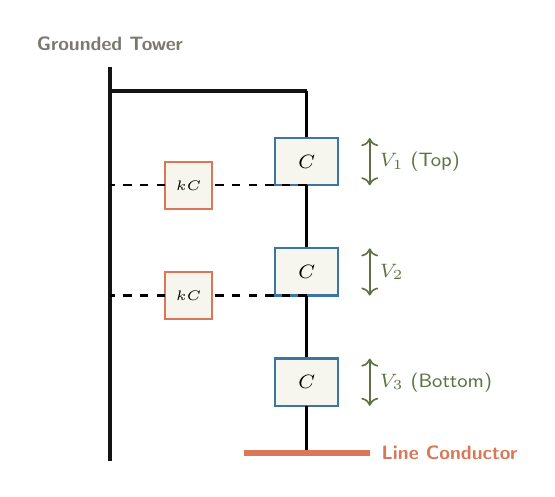
\begin{tikzpicture}[scale=1.0]
  %% Tower Ground
  \draw[line width=1.5pt, color=AnthDark] (-2.5, 4.5) -- (-2.5, -0.5);
  \node[font=\scriptsize\sffamily\bfseries, color=AnthMidGray] at (-2.5, 4.8) {Grounded Tower};

  %% Crossarm
  \draw[line width=1.5pt, color=AnthDark] (-2.5, 4.2) -- (0, 4.2);

  %% Capacitors String
  \draw[line width=1.0pt] (0, 4.2) -- (0, 3.6);
  \draw[draw=AnthBlue, fill=AnthCardBG, line width=0.8pt] (-0.4, 3.0) rectangle (0.4, 3.6) node[midway, font=\scriptsize\sffamily\bfseries]{$C$};
  \draw[line width=1.0pt] (0, 3.0) -- (0, 2.2);
  \draw[draw=AnthBlue, fill=AnthCardBG, line width=0.8pt] (-0.4, 1.6) rectangle (0.4, 2.2) node[midway, font=\scriptsize\sffamily\bfseries]{$C$};
  \draw[line width=1.0pt] (0, 1.6) -- (0, 0.8);
  \draw[draw=AnthBlue, fill=AnthCardBG, line width=0.8pt] (-0.4, 0.2) rectangle (0.4, 0.8) node[midway, font=\scriptsize\sffamily\bfseries]{$C$};
  \draw[line width=1.0pt] (0, 0.2) -- (0, -0.4);

  %% Shunt Capacitors to Ground
  \draw[line width=0.8pt, dashed] (0, 3.0) -- (-1.2, 3.0);
  \draw[draw=AnthOrange, fill=AnthCardBG, line width=0.7pt] (-1.8, 2.7) rectangle (-1.2, 3.3) node[midway, font=\tiny\sffamily]{$kC$};
  \draw[line width=0.8pt, dashed] (-1.8, 3.0) -- (-2.5, 3.0);

  \draw[line width=0.8pt, dashed] (0, 1.6) -- (-1.2, 1.6);
  \draw[draw=AnthOrange, fill=AnthCardBG, line width=0.7pt] (-1.8, 1.3) rectangle (-1.2, 1.9) node[midway, font=\tiny\sffamily]{$kC$};
  \draw[line width=0.8pt, dashed] (-1.8, 1.6) -- (-2.5, 1.6);

  %% Conductor at Bottom
  \draw[line width=2.0pt, color=AnthOrange] (-0.8, -0.4) -- (0.8, -0.4) node[right, font=\scriptsize\sffamily\bfseries]{Line Conductor};

  %% Voltage Annotations
  \draw[<->, line width=0.6pt, color=AnthGreen] (0.8, 3.6) -- node[right, font=\scriptsize\sffamily]{$V_1$ (Top)} (0.8, 3.0);
  \draw[<->, line width=0.6pt, color=AnthGreen] (0.8, 2.2) -- node[right, font=\scriptsize\sffamily]{$V_2$} (0.8, 1.6);
  \draw[<->, line width=0.6pt, color=AnthGreen] (0.8, 0.8) -- node[right, font=\scriptsize\sffamily]{$V_3$ (Bottom)} (0.8, 0.2);
\end{tikzpicture}%
}
\end{center}

\begin{Deriv}[Mathematical Derivation of Disc Voltages (3-Unit String)]
Let $V_1, V_2, V_3$ be voltages across top, middle, and bottom discs, and $\omega$ be angular frequency.
Applying Kirchhoff's Current Law (KCL) at each intermediate node:

1. 	extbf{At Node 1 (between Disc 1 and Disc 2):}
\begin{equation}
  I_2 = I_1 + i_1 \implies V_2 (\omega C) = V_1 (\omega C) + V_1 (\omega k C) \implies V_2 = V_1 (1 + k)
\end{equation}

2. 	extbf{At Node 2 (between Disc 2 and Disc 3):}
The potential of Node 2 above ground is $V_1 + V_2$.
\begin{align}
  I_3 &= I_2 + i_2 \implies V_3 (\omega C) = V_2 (\omega C) + (V_1 + V_2)(\omega k C) \nonumber\\
  V_3 &= V_2 + k (V_1 + V_2) = V_1 (1 + k) + k [V_1 + V_1(1 + k)] = V_1 \left( 1 + 3k + k^2 \right)
\end{align}

3. 	extbf{Total Phase-to-Ground Voltage ($V$):}
\begin{align}
  V &= V_1 + V_2 + V_3 = V_1 + V_1(1 + k) + V_1(1 + 3k + k^2) \nonumber\\
    &= V_1 \left( 3 + 4k + k^2 \right)
\end{align}
\end{Deriv}

\begin{Tip}[Key Observation: Non-Uniform Voltage Distribution]
Since $k > 0$, it follows that $V_1 < V_2 < V_3$. The disc 	extbf{nearest to the energized line conductor ($V_3$) experiences the maximum electrical voltage stress} and is most prone to dielectric puncture or flashover.
\end{Tip}

%% ─────────────────────────────────────────────────────────────────────────────
\subsection{String Efficiency and Methods of Improvement}

\begin{Def}[String Efficiency ($\eta_{\text{string}}$)]
String efficiency is the ratio of total phase voltage across the string to the product of the number of discs and the voltage across the lowest disc:
\begin{equation}
  \eta_{\text{string}} = \frac{\text{Total Voltage Across String ($V$)}}{n \times \text{Voltage Across Disc Nearest to Conductor ($V_n$)}} \times 100\%
\end{equation}
\end{Def}

\concept{Methods of Equalizing Voltage Distribution (Improving $\eta_{\text{string}}$)}
\begin{enumerate}
  \item \textbf{Using Longer Cross-Arms:} Increasing tower clearance reduces shunt capacitance $C_1$, decreasing the ratio $k = C_1 / C$. However, tower structural weight and cost limit this approach.
  \item \textbf{Capacitance Grading of Discs:} Using insulator discs of varying capacitance. Discs with larger mutual capacitance $C$ are placed near conductor end so that $V = \frac{I}{\omega C}$ remains equal across all units.
  \item \textbf{Static Shield / Guard Ring:} A conductive metallic ring connected directly to the high-voltage conductor surrounding the bottom unit. The ring introduces 	extbf{shielding capacitances ($C_2$)} between the energized conductor and the link pins, injecting currents that neutralize shunt leakage currents to ground, producing \textbf{100\% uniform voltage distribution}.
\end{enumerate}

%% ─────────────────────────────────────────────────────────────────────────────
\clearpage
\section{Comprehensive Numerical Problem Suite}
%% ─────────────────────────────────────────────────────────────────────────────

\begin{Problem}[Problem 1: Inductance of a Symmetrically Transposed 3-$\Phi$ Single Circuit Line]
A $3$-phase, $50\,\text{Hz}$, $132\,\text{kV}$ transmission line has conductors of diameter $2.0\,\text{cm}$ placed at the corners of a triangle with sides $3\,\text{m}$, $4\,\text{m}$, and $5\,\text{m}$. If the line is regularly transposed, calculate: (a) Self GMR, (b) Mutual GMD, (c) Inductance per phase per km, and (d) Inductive reactance per phase for a $100\,\text{km}$ line length.
\end{Problem}

\begin{Solution}
\begin{enumerate}
  \item Conductor radius: $r = \frac{2.0}{2} = 1.0\,\text{cm} = 0.01\,\text{m}$.
  \item Self GMR: $D_s = r' = 0.7788 \times 0.01 = \mathbf{0.007788\,\text{m}} = 7.788\,\text{mm}$.
  \item Mutual GMD:
    \begin{align*}
      D_m &= \sqrt[3]{D_{12} \cdot D_{23} \cdot D_{31}} = \sqrt[3]{3 \times 4 \times 5} = \sqrt[3]{60} = \mathbf{3.9149\,\text{m}}
    \end{align*}
  \item Inductance per phase per meter:
    \begin{align*}
      L &= 2 \times 10^{-7} \ln\left(\frac{D_m}{D_s}\right) = 2 \times 10^{-7} \ln\left(\frac{3.9149}{0.007788}\right) \\
        &= 2 \times 10^{-7} \ln(502.68) = 2 \times 10^{-7} \times 6.22 = \mathbf{1.244 \times 10^{-6}\,\text{H/m}} = \mathbf{1.244\,\text{mH/km/phase}}
    \end{align*}
  \item Inductive Reactance for $100\,\text{km}$:
    \begin{align*}
      X_L &= 2\pi f L \times 100 = 2\pi \times 50 \times (1.244 \times 10^{-3}) \times 100 = \mathbf{39.08\,\Omega/\text{phase}}
    \end{align*}
\end{enumerate}
\end{Solution}

\begin{Problem}[Problem 2: Capacitance of a 3-$\Phi$ Transposed Single Circuit Line]
For the transmission line in Problem 1, calculate: (a) Line-to-neutral capacitance per km, (b) Line-to-line capacitance per km, and (c) Charging current per km at $132\,\text{kV}$.
\end{Problem}

\begin{Solution}
\begin{enumerate}
  \item Actual radius: $r = 0.01\,\text{m}$, $D_m = 3.9149\,\text{m}$.
  \item Line-to-neutral capacitance:
    \begin{align*}
      C_n &= \frac{2\pi \epsilon_0}{\ln(D_m / r)} = \frac{2\pi \times 8.854 \times 10^{-12}}{\ln(3.9149 / 0.01)} = \frac{5.5635 \times 10^{-11}}{\ln(391.49)} \\
          &= \frac{5.5635 \times 10^{-11}}{5.97} = \mathbf{9.319 \times 10^{-12}\,\text{F/m}} = \mathbf{0.00932\,\mu\text{F/km/phase}}
    \end{align*}
  \item Line-to-line capacitance: $C_{ab} = \frac{C_n}{2} = \mathbf{0.00466\,\mu\text{F/km}}$.
  \item Operating phase voltage: $V_{\text{ph}} = \frac{132 \times 10^3}{\sqrt{3}} = 76,210.23\,\text{V}$.
  \item Charging current per km:
    \begin{align*}
      I_c &= \omega C_n V_{\text{ph}} = 2\pi \times 50 \times (9.319 \times 10^{-9}\,\text{F/km}) \times 76,210.23 = \mathbf{0.223\,\text{A/km}}
    \end{align*}
\end{enumerate}
\end{Solution}

\begin{Problem}[Problem 3: Inductance of a Three-Phase Double-Circuit Line]
A $3$-phase double-circuit line has vertical flat configuration with conductor diameter $2.5\,\text{cm}$. The spacing between vertically adjacent conductors of the same circuit is $4\,\text{m}$. The horizontal distance between the two circuits is $6\,\text{m}$. The phase arrangement is $a-b-c$ on Circuit 1 and $c'-b'-a'$ on Circuit 2. Calculate the inductance per phase per km.
\end{Problem}

\begin{Solution}
\begin{enumerate}
  \item Coordinates: $a(-3, 4)$, $b(-3, 0)$, $c(-3, -4)$, and $c'(3, 4)$, $b'(3, 0)$, $a'(3, -4)$.
  \item Conductor parameters: $r = \frac{2.5}{2} = 1.25\,\text{cm} = 0.0125\,\text{m}$, $r' = 0.7788 \times 0.0125 = 0.009735\,\text{m}$.
  \item Distances between paired conductors:
    \begin{align*}
      D_{aa'} &= \sqrt{(6)^2 + (8)^2} = \sqrt{36 + 64} = 10\,\text{m}, \quad D_{bb'} = 6\,\text{m}, \quad D_{cc'} = 10\,\text{m}
    \end{align*}
  \item Self GMD of individual phases:
    \begin{align*}
      D_{sa} &= \sqrt{r' \cdot D_{aa'}} = \sqrt{0.009735 \times 10} = 0.3120\,\text{m} \\
      D_{sb} &= \sqrt{r' \cdot D_{bb'}} = \sqrt{0.009735 \times 6} = 0.2417\,\text{m}, \quad D_{sc} = 0.3120\,\text{m} \\
      D_s &= \sqrt[3]{0.3120 \times 0.2417 \times 0.3120} = \mathbf{0.2865\,\text{m}}
    \end{align*}
  \item Mutual GMD between phases:
    \begin{align*}
      D_{ab} &= \sqrt[4]{4 \times \sqrt{6^2 + 4^2} \times \sqrt{6^2 + 4^2} \times 4} = \sqrt{4 \times 7.2111} = 5.3707\,\text{m} \\
      D_{bc} &= 5.3707\,\text{m} \\
      D_{ca} &= \sqrt[4]{8 \times 6 \times 6 \times 8} = \sqrt{48} = 6.9282\,\text{m} \\
      D_m &= \sqrt[3]{5.3707 \times 5.3707 \times 6.9282} = \mathbf{5.8465\,\text{m}}
    \end{align*}
  \item Inductance per phase:
    \begin{align*}
      L &= 2 \times 10^{-7} \ln\left(\frac{D_m}{D_s}\right) = 2 \times 10^{-7} \ln\left(\frac{5.8465}{0.2865}\right) \\
        &= 2 \times 10^{-7} \ln(20.407) = 2 \times 10^{-7} \times 3.0159 = \mathbf{0.603\,\text{mH/km/phase}}
    \end{align*}
\end{enumerate}
\end{Solution}

\begin{Problem}[Problem 4: ABCD Parameters of a Medium Nominal-T Transmission Line]
A 3-phase, $50\,\text{Hz}$, $100\,\text{km}$ transmission line has total series impedance $Z = 20 + j40\,\Omega$ and total shunt admittance $Y = j 3 \times 10^{-4}\,\mho$. Determine the ABCD constants of the Nominal-T network and verify reciprocity.
\end{Problem}

\begin{Solution}
\begin{enumerate}
  \item Product $YZ$:
    \begin{equation*}
      YZ = (j 3 \times 10^{-4})(20 + j40) = -0.012 + j 0.006
    \end{equation*}
  \item Parameter $A$ and $D$:
    \begin{align*}
      A = D &= 1 + \frac{YZ}{2} = 1 + \frac{-0.012 + j0.006}{2} \\
            &= 0.994 + j 0.003 = \mathbf{0.9940 \angle 0.173^\circ}
    \end{align*}
  \item Parameter $B$:
    \begin{align*}
      B &= Z \left(1 + \frac{YZ}{4}\right) = (20 + j40) \left(0.997 + j0.0015\right) \\
        &= 19.88 + j 39.91\,\Omega = \mathbf{44.59 \angle 63.52^\circ\,\Omega}
    \end{align*}
  \item Parameter $C$:
    \begin{equation*}
      C = Y = \mathbf{j 3 \times 10^{-4}\,\mho} = \mathbf{0.0003 \angle 90^\circ\,\mho}
    \end{equation*}
  \item Verification of Reciprocity ($AD - BC = 1$):
    \begin{align*}
      AD - BC &= (0.994 + j0.003)^2 - (19.88 + j39.91)(j 0.0003) \\
              &= (0.988027 + j 0.005964) - (j 0.005964 - 0.011973) = \mathbf{1.0000} \quad \checkmark
    \end{align*}
\end{enumerate}
\end{Solution}

\begin{Problem}[Problem 5: Performance and Voltage Regulation of Nominal-$\pi$ Line]
A 3-phase, $132\,\text{kV}$, $50\,\text{Hz}$ line delivers $50\,\text{MW}$ at $0.8$ power factor lagging at $132\,\text{kV}$. Total line parameters: $Z = 25 + j 60\,\Omega$, $Y = j 4 \times 10^{-4}\,\mho$. Using the Nominal-$\pi$ model, calculate: (a) Sending-end voltage, (b) Sending-end current, (c) Voltage regulation, and (d) Transmission efficiency.
\end{Problem}

\begin{Solution}
\begin{enumerate}
  \item Receiving-end phase voltage: $V_r = \frac{132 \times 10^3}{\sqrt{3}} = 76,210.23 \angle 0^\circ\,\text{V}$.
  \item Receiving-end line current:
    \begin{equation*}
      |I_r| = \frac{50 \times 10^6}{\sqrt{3} \times 132 \times 10^3 \times 0.8} = 273.37\,\text{A} \implies I_r = 273.37 \angle -36.87^\circ = (218.70 - j 164.02)\,\text{A}
    \end{equation*}
  \item ABCD Parameters (Nominal-$\pi$):
    \begin{align*}
      A = D &= 1 + \frac{YZ}{2} = 0.988 + j 0.005 = 0.9880 \angle 0.29^\circ \\
      B &= Z = 25 + j 60\,\Omega = 65.0 \angle 67.38^\circ\,\Omega \\
      C &= Y \left(1 + \frac{YZ}{4}\right) \approx j 3.976 \times 10^{-4}\,\mho
    \end{align*}
  \item Sending-End Voltage ($V_s$):
    \begin{align*}
      V_s &= A V_r + B I_r = (0.988 + j0.005)(76210.23) + (25 + j60)(218.70 - j164.02) \\
          &= 90604.4 + j 9402.6 = \mathbf{91,091.2 \angle 5.92^\circ\,\text{V/phase}}
    \end{align*}
    $V_{s,\text{line}} = \sqrt{3} \times 91,091.2 = \mathbf{157.77\,\text{kV}}$.
  \item Sending-End Current ($I_s$):
    \begin{align*}
      I_s &= C V_r + D I_r = (j 3.976 \times 10^{-4})(76210.23) + (0.988 + j0.005)(218.70 - j164.02) \\
          &= 216.90 - j 130.66 = \mathbf{253.24 \angle -31.06^\circ\,\text{A}}
    \end{align*}
  \item Percentage Voltage Regulation:
    \begin{align*}
      \% VR &= \frac{|V_s / A| - |V_r|}{|V_r|} \times 100\% = \frac{\frac{91,091.2}{0.988} - 76,210.23}{76,210.23} \times 100\% = \mathbf{20.98\%}
    \end{align*}
  \item Transmission Efficiency ($\eta\%$):
    \begin{align*}
      P_s &= 3 \operatorname{Re}(V_s \cdot I_s^*) = 3 \times |V_s| |I_s| \cos(5.92^\circ - (-31.06^\circ)) \\
          &= 3 \times 91091.2 \times 253.24 \times \cos(36.98^\circ) = \mathbf{55.29\,\text{MW}} \\
      \eta &= \frac{P_r}{P_s} \times 100\% = \frac{50}{55.29} \times 100\% = \mathbf{90.43\%}
    \end{align*}
\end{enumerate}
\end{Solution}

\begin{Problem}[Problem 6: String Efficiency of a 3-Disc Suspension Insulator String]
In a 3-unit suspension insulator string, the shunt capacitance between each link pin and earth is $15\%$ of the self-capacitance of each unit ($k = 0.15$). If the total working voltage across the string is $33\,\text{kV}$, calculate: (a) Voltage distribution across each disc, and (b) String efficiency.
\end{Problem}

\begin{Solution}
\begin{enumerate}
  \item Disc Voltage Relationships:
    \begin{align*}
      V_2 &= V_1 (1 + k) = V_1 (1 + 0.15) = \mathbf{1.15\,V_1} \\
      V_3 &= V_1 (1 + 3k + k^2) = V_1 (1 + 0.45 + 0.0225) = \mathbf{1.4725\,V_1}
    \end{align*}
  \item Total string voltage equation:
    \begin{equation*}
      V = V_1 + V_2 + V_3 = V_1 (1 + 1.15 + 1.4725) = 3.6225\,V_1 = 33\,\text{kV}
    \end{equation*}
  \item Voltage across individual discs:
    \begin{align*}
      V_1 &= \frac{33}{3.6225} = \mathbf{9.110\,\text{kV}} \quad (\text{Top Unit}) \\
      V_2 &= 1.15 \times 9.110 = \mathbf{10.476\,\text{kV}} \quad (\text{Middle Unit}) \\
      V_3 &= 1.4725 \times 9.110 = \mathbf{13.414\,\text{kV}} \quad (\text{Bottom Unit nearest to conductor})
    \end{align*}
  \item String Efficiency:
    \begin{equation*}
      \eta_{\text{string}} = \frac{V}{n \times V_3} \times 100\% = \frac{33}{3 \times 13.414} \times 100\% = \frac{33}{40.242} \times 100\% = \mathbf{82.00\%}
    \end{equation*}
\end{enumerate}
\end{Solution}

\begin{Problem}[Problem 7: Capacitance Grading for 100\% String Efficiency]
A 4-unit suspension insulator string has a shunt-to-mutual capacitance ratio $k = 0.1$ for standard units of mutual capacitance $C$. If the voltage across every disc is to be made identical ($V_1 = V_2 = V_3 = V_4 = V/4$), calculate the graded mutual capacitances $C_1, C_2, C_3, C_4$ in terms of $C$.
\end{Problem}

\begin{Solution}
For equal voltage distribution $V_1 = V_2 = V_3 = V_4 = v$:
\begin{enumerate}
  \item Top unit: $C_1 = C$.
  \item Current in unit 2: $I_2 = I_1 + i_1 \implies v \omega C_2 = v \omega C_1 + v \omega (0.1 C) \implies C_2 = C_1 + 0.1 C = \mathbf{1.1\,C}$.
  \item Current in unit 3: $I_3 = I_2 + i_2 \implies v \omega C_3 = v \omega C_2 + 2v \omega (0.1 C) \implies C_3 = C_2 + 0.2 C = 1.1C + 0.2C = \mathbf{1.3\,C}$.
  \item Current in unit 4: $I_4 = I_3 + i_3 \implies v \omega C_4 = v \omega C_3 + 3v \omega (0.1 C) \implies C_4 = C_3 + 0.3 C = 1.3C + 0.3C = \mathbf{1.6\,C}$.
  \item \textbf{Required Grading Ratio:} $C_1 : C_2 : C_3 : C_4 = \mathbf{1.0 : 1.1 : 1.3 : 1.6}$.
\end{enumerate}
\end{Solution}

\begin{Problem}[Problem 8: Sizing Guard Ring Shielding Capacitance]
A 3-unit suspension string has shunt capacitance $C_1 = 0.2\,C$. A guard ring is fitted to equalize the voltages across the bottom two units ($V_2 = V_3$). Find the required shielding capacitance $C_2$ between the guard ring and the lower intermediate pin.
\end{Problem}

\begin{Solution}
Let voltage across top unit be $V_1$.
\begin{enumerate}
  \item At Node 1 (no guard ring connection): $V_2 = V_1 (1 + 0.2) = 1.2\,V_1$.
  \item At Node 2: The guard ring connected to the line conductor ($V$) injects current $i_{\text{guard}} = (V - (V_1 + V_2))\omega C_2 = V_3 \omega C_2$.
  \item KCL at Node 2:
    \begin{equation*}
      I_3 + i_{\text{guard}} = I_2 + i_2 \implies V_3 \omega C + V_3 \omega C_2 = V_2 \omega C + (V_1 + V_2)\omega (0.2 C)
    \end{equation*}
  \item Imposing $V_2 = V_3 = 1.2\,V_1$:
    \begin{align*}
      1.2 V_1 C + 1.2 V_1 C_2 &= 1.2 V_1 C + (V_1 + 1.2 V_1)(0.2 C) \\
      1.2 C_2 &= 2.2 \times 0.2 C = 0.44 C \implies C_2 = \frac{0.44}{1.2} C = \mathbf{0.367\,C}
    \end{align*}
\end{enumerate}
\end{Solution}

\begin{Problem}[Problem 9: Surge Impedance Loading of a 400 kV Line]
A $400\,\text{kV}$, 3-phase transmission line has series inductance $L = 1.05\,\text{mH/km}$ and shunt capacitance $C = 0.011\,\mu\text{F/km}$. Calculate: (a) Surge Impedance ($Z_c$), (b) Surge Impedance Loading (SIL), and (c) New SIL if bundle conductor modifications decrease $L$ by $10\%$ and increase $C$ by $15\%$.
\end{Problem}

\begin{Solution}
\begin{enumerate}
  \item Surge Impedance:
    \begin{align*}
      Z_c &= \sqrt{\frac{L}{C}} = \sqrt{\frac{1.05 \times 10^{-3}}{0.011 \times 10^{-6}}} = \sqrt{95,454.55} = \mathbf{308.96\,\Omega}
    \end{align*}
  \item Surge Impedance Loading (SIL):
    \begin{align*}
      \text{SIL} &= \frac{V_{\text{L-L}}^2}{Z_c} = \frac{(400 \times 10^3)^2}{308.96} = \frac{160,000 \times 10^6}{308.96} = \mathbf{517.87\,\text{MW}}
    \end{align*}
  \item Modified parameters: $L_{\text{new}} = 0.90 \times 1.05 = 0.945\,\text{mH/km}$, $C_{\text{new}} = 1.15 \times 0.011 = 0.01265\,\mu\text{F/km}$.
    \begin{align*}
      Z_{c,\text{new}} &= \sqrt{\frac{0.945 \times 10^{-3}}{0.01265 \times 10^{-6}}} = \sqrt{74,703.56} = \mathbf{273.32\,\Omega} \\
      \text{SIL}_{\text{new}} &= \frac{(400)^2}{273.32} = \mathbf{585.39\,\text{MW}} \quad (\text{13.04\% Capacity Increase})
    \end{align*}
\end{enumerate}
\end{Solution}

\begin{Problem}[Problem 10: Critical Disruptive Voltage and Visual Corona Calculation]
A 3-phase, $220\,\text{kV}$, $50\,\text{Hz}$ line has stranded conductors of diameter $2.2\,\text{cm}$ spaced equilaterally at $3.5\,\text{m}$. Barometric pressure is $74\,\text{cm of Hg}$ and temperature is $30^\circ\text{C}$. Conductor irregularity factor $m_0 = 0.85$, $m_v = 0.72$, and breakdown strength of air $g_0 = 21.2\,\text{kV/cm (rms)}$. Calculate: (a) Air density correction factor, (b) Critical disruptive voltage, and (c) Visual critical voltage.
\end{Problem}

\begin{Solution}
\begin{enumerate}
  \item Conductor radius: $r = \frac{2.2}{2} = 1.1\,\text{cm}$, spacing $d = 350\,\text{cm}$.
  \item Air density correction factor:
    \begin{equation*}
      \delta = \frac{3.92 b}{273 + t} = \frac{3.92 \times 74}{273 + 30} = \frac{290.08}{303} = \mathbf{0.9574}
    \end{equation*}
  \item Critical Disruptive Voltage (Line-to-neutral):
    \begin{align*}
      V_d &= m_0 g_0 \delta r \ln\left(\frac{d}{r}\right) = (0.85) \times (21.2) \times (0.9574) \times (1.1) \times \ln\left(\frac{350}{1.1}\right) \\
          &= 18.976 \times \ln(318.18) = 18.976 \times 5.7626 = \mathbf{109.35\,\text{kV/phase rms}}
    \end{align*}
    $V_{d,\text{line}} = \sqrt{3} \times 109.35 = \mathbf{189.40\,\text{kV}}$.
  \item Visual Critical Voltage (Line-to-neutral):
    \begin{align*}
      V_v &= m_v g_0 \delta r \left( 1 + \frac{0.3}{\sqrt{\delta r}} \right) \ln\left(\frac{d}{r}\right) \\
          &= 16.074 \times \left( 1 + \frac{0.3}{\sqrt{0.9574 \times 1.1}} \right) \times 5.7626 = \mathbf{119.70\,\text{kV/phase rms}}
    \end{align*}
    $V_{v,\text{line}} = \sqrt{3} \times 119.70 = \mathbf{207.33\,\text{kV}}$.
  \item \textbf{Operational Conclusion:} Operating voltage ($220\,\text{kV}$) exceeds both $V_d$ ($189.4\,\text{kV}$) and $V_v$ ($207.3\,\text{kV}$), meaning 	extbf{visible corona and power loss will occur}.
\end{enumerate}
\end{Solution}

\begin{Problem}[Problem 11: Corona Power Loss Evaluation using Peek's Formula]
For the transmission line in Problem 10, operating at $220\,\text{kV}$ line-to-line over a length of $150\,\text{km}$, calculate the total 3-phase active corona power loss under fair weather conditions.
\end{Problem}

\begin{Solution}
\begin{enumerate}
  \item Operating phase voltage: $V_{\text{ph}} = \frac{220}{\sqrt{3}} = 127.02\,\text{kV}$.
  \item Critical disruptive phase voltage: $V_d = 109.35\,\text{kV}$.
  \item Voltage excess: $V_{\text{ph}} - V_d = 127.02 - 109.35 = 17.67\,\text{kV}$.
  \item Peek's Formula per phase per km:
    \begin{align*}
      P &= \frac{242.2}{\delta} (f + 25) \sqrt{\frac{r}{d}} (V_{\text{ph}} - V_d)^2 \times 10^{-5} \\
        &= \frac{242.2}{0.9574} (50 + 25) \sqrt{\frac{1.1}{350}} (17.67)^2 \times 10^{-5} = \mathbf{3.321\,\text{kW/km/phase}}
    \end{align*}
  \item Total 3-Phase Power Loss for $150\,\text{km}$:
    \begin{equation*}
      P_{\text{total}} = 3 \times 3.321 \times 150 = \mathbf{1,494.45\,\text{kW}} \approx \mathbf{1.49\,\text{MW}}
    \end{equation*}
\end{enumerate}
\end{Solution}

\begin{Problem}[Problem 12: Ferranti Rise on an Unloaded Long Transmission Line]
A 3-phase, $400\,\text{kV}$, $50\,\text{Hz}$, $300\,\text{km}$ lossless transmission line has distributed parameters $L = 1.0\,\text{mH/km}$ and $C = 0.01\,\mu\text{F/km}$. If the sending-end voltage is held constant at $400\,\text{kV}$, determine: (a) No-load receiving-end voltage, and (b) Rating of shunt reactor required to restore receiving-end voltage to $400\,\text{kV}$.
\end{Problem}

\begin{Solution}
\begin{enumerate}
  \item Phase propagation constant ($\beta$):
    \begin{align*}
      \beta &= \omega \sqrt{L C} = 2\pi \times 50 \times \sqrt{(1.0 \times 10^{-3})(0.01 \times 10^{-6})} = 9.934 \times 10^{-4}\,\text{rad/km} \\
      \theta &= \beta l = (9.934 \times 10^{-4}) \times 300 = \mathbf{0.2980\,\text{rad}} = \mathbf{17.075^\circ}
    \end{align*}
  \item Parameter $A = \cos(\beta l) = \cos(17.075^\circ) = \mathbf{0.9559}$.
  \item No-load receiving-end voltage ($I_r = 0$):
    \begin{equation*}
      V_{r0} = \frac{V_s}{A} = \frac{400\,\text{kV}}{0.9559} = \mathbf{418.45\,\text{kV (Line-to-Line)}} \quad (\text{Voltage Rise } = 18.45\,\text{kV})
    \end{equation*}
  \item Surge Impedance: $Z_c = \sqrt{\frac{L}{C}} = \sqrt{\frac{1.0 \times 10^{-3}}{0.01 \times 10^{-6}}} = \mathbf{316.23\,\Omega}$.
  \item Shunt Reactor Requirement:
    \begin{align*}
      X_{\text{reactor}} &= \frac{Z_c \sin(\beta l)}{1 - A} = \frac{316.23 \times \sin(17.075^\circ)}{1 - 0.9559} = \frac{316.23 \times 0.2936}{0.0441} = \mathbf{2,105.3\,\Omega/\text{phase}}
    \end{align*}
  \item Total 3-Phase Shunt Reactor Rating:
    \begin{equation*}
      Q_{\text{reactor}} = \frac{V_{\text{L-L}}^2}{X_{\text{reactor}}} = \frac{(400 \times 10^3)^2}{2105.3} = \mathbf{76.0\,\text{MVAR}}
    \end{equation*}
\end{enumerate}
\end{Solution}

%% ─────────────────────────────────────────────────────────────────────────────
\clearpage
\section{Quick Revision Sheet \& Model Examination Questions}
%% ─────────────────────────────────────────────────────────────────────────────

\subsection{Master Formula Summary Table for Module 2}

\begin{center}
\small
\begin{tabularx}{\textwidth}{L{3.2cm} L{5.2cm} X}
  \rowcolor{AnthDark}
  \color{white}\textbf{Topic / Phenomenon} & \color{white}\textbf{Governing Mathematical Formula} & \color{white}\textbf{Physical Significance} \\
  \rowcolor{AnthCardBG} \textbf{Line Inductance} & $L = 2\times 10^{-7} \ln\left(\frac{D_m}{D_s}\right)\,\text{H/m/phase}$ & Self GMR $D_s = 0.7788r$ accounts for internal flux linkages \\
  \textbf{Line Capacitance} & $C_n = \frac{2\pi \epsilon_0}{\ln(D_m / D_{sc})}\,\text{F/m/phase}$ & Uses actual physical radius $r$ (surface charge) \\
  \rowcolor{AnthCardBG} \textbf{Two-Port Equations} & $V_s = A V_r + B I_r, \quad I_s = C V_r + D I_r$ & Symmetric ($A=D$), Reciprocal ($AD-BC=1$) \\
  \textbf{Nominal-T Model} & $A = 1+\frac{YZ}{2}, \, B = Z(1+\frac{YZ}{4}), \, C=Y$ & Middle lumped shunt admittance \\
  \rowcolor{AnthCardBG} \textbf{Nominal-$\pi$ Model} & $A = 1+\frac{YZ}{2}, \, B = Z, \, C=Y(1+\frac{YZ}{4})$ & Shunt admittance split $Y/2$ at ends \\
  \textbf{Voltage Regulation} & $\%VR = \frac{|V_s/A| - |V_r|}{|V_r|} \times 100\%$ & Percentage receiving voltage drop on full load \\
  \rowcolor{AnthCardBG} \textbf{Ferranti Effect} & $V_r - V_s \approx \frac{V_r \omega^2 l^2 L C}{2} > 0$ & No-load receiving overvoltage; mitigated by shunt reactors \\
  \textbf{Critical Disruptive} & $V_d = m_0 g_0 \delta r \ln(d/r)\,\text{kV/phase}$ & Breakdown of air surrounding high voltage conductors \\
  \rowcolor{AnthCardBG} \textbf{Surge Impedance} & $Z_c = \sqrt{L/C}, \quad \text{SIL} = \frac{V_{\text{L-L}}^2}{Z_c}$ & Flat voltage profile and zero net reactive exchange at SIL \\
  \textbf{String Efficiency} & $\eta = \frac{V}{n \times V_n} \times 100\%$ & Voltage non-uniformity across suspension insulator discs \\
\end{tabularx}
\end{center}

\subsection{Model Examination Questions (KTU S5 Pattern)}

\begin{Warn}[University Examination Pattern (PCEOT503 Scheme)]
The End Semester Examination consists of \textbf{Part A} (8 compulsory questions of 3 marks each, 2 from each module) and \textbf{Part B} (Module choice questions carrying 9 marks each).
\end{Warn}

\concept{Part A: Short Answer Questions (3 Marks Each)}
\begin{enumerate}
  \item \textbf{Q1:} Define \emph{Skin Effect}. Explain why stranded ACSR conductors mitigate skin effect in power transmission.
  \item \textbf{Q2:} What is \emph{Ferranti Effect}? Draw the phasor diagram under no-load condition and name the equipment used for its mitigation.
  \item \textbf{Q3:} State the physical significance of \emph{Surge Impedance Loading (SIL)}. What happens when a line operates above SIL?
  \item \textbf{Q4:} Why is the fictitious radius $r' = 0.7788r$ used in inductance calculation but not in capacitance calculation?
  \item \textbf{Q5:} Define \emph{String Efficiency} of an insulator string. Why is voltage distribution across suspension discs non-uniform?
  \item \textbf{Q6:} State the conditions for symmetry and reciprocity in terms of transmission line ABCD parameters.
\end{enumerate}

\concept{Part B: Long Answer / Analytical Questions (9 Marks Each)}
\begin{enumerate}
  \item \textbf{Q7 (a):} Derive the expression for the loop inductance per phase of a transposed three-phase double-circuit line using the GMD and GMR method. \hfill (6 Marks) \\
  \textbf{Q7 (b):} Explain the advantages of bundled conductors over single solid conductors in EHV lines. \hfill (3 Marks)
  
  \item \textbf{Q8 (a):} Derive the ABCD parameters for a medium transmission line using the Nominal-$\pi$ method and show that $AD - BC = 1$. \hfill (5 Marks) \\
  \textbf{Q8 (b):} A 3-phase, $50\,\text{Hz}$, $132\,\text{kV}$ transmission line delivers $40\,\text{MW}$ at $0.8$ power factor lagging. The ABCD parameters are $A = D = 0.98 \angle 0.5^\circ$, $B = 60 \angle 70^\circ\,\Omega$, $C = 0.0004 \angle 90^\circ\,\mho$. Calculate the sending-end voltage and percentage voltage regulation. \hfill (4 Marks)

  \item \textbf{Q9 (a):} Derive the mathematical expressions for the voltage distribution across a 3-unit suspension insulator string and obtain the expression for string efficiency. \hfill (5 Marks) \\
  \textbf{Q9 (b):} Discuss the methods used for improving string efficiency. Explain how a guard ring produces uniform voltage distribution. \hfill (4 Marks)
\end{enumerate}

\vfill
\begin{center}
\small\sffamily\color{AnthMidGray}
--- End of Module 2 Study Notes ---
\end{center}

\end{document}
